% Document principal : compiler ce fichier avec pdfLaTeX, trois fois.
\documentclass[11pt,a4paper]{report}
% Préambule du rapport : compilation depuis main.tex.
% Les textes de couverture et les couleurs peuvent être modifiés ci-dessous.
\usepackage[T1]{fontenc}
\usepackage[utf8]{inputenc}
\IfFileExists{french.ldf}{%
  \usepackage[french]{babel}
}{%
  \usepackage{babel}
  \babelprovide[main,import]{french}
}
\usepackage{lmodern}
\usepackage{microtype}
\usepackage[a4paper,left=23mm,right=23mm,top=25mm,bottom=21mm]{geometry}
\usepackage{graphicx}
\usepackage{xcolor}
\usepackage{amsmath,amssymb}
\usepackage{booktabs,tabularx,array,longtable}
\usepackage{ragged2e}
\usepackage{caption}
\usepackage{placeins}
\usepackage{titlesec}
\usepackage{tikz}
\usetikzlibrary{arrows.meta,positioning}
\usepackage{hyperref}
\setlength{\parindent}{0pt}

\definecolor{anthracite}{HTML}{252728}
\definecolor{terreCuite}{HTML}{A5553E}
\definecolor{grisTexte}{HTML}{62666A}
\definecolor{grisCredit}{HTML}{7B7E81}
\newcolumntype{L}{>{\raggedright\arraybackslash}X}
\newcommand{\nomChapitre}{CHAPITRE}
\newcommand{\code}[1]{{\ttfamily\small\detokenize{#1}}}
\newcommand{\sourcecalcul}[1]{\par\vspace{2pt}{\footnotesize\color{grisTexte}Source : #1.\par}}
\newcommand{\bilan}[1]{\par\medskip\noindent{\sffamily\bfseries À retenir. }#1\par}
\newcommand{\figurerapport}[4][0.98]{%
  \begin{figure}[htbp]\centering
  \includegraphics[width=#1\textwidth]{figures/#2}
  \caption{#3}\label{#4}
  \sourcecalcul{calculs du projet, données BAAC ; notebooks 04 et 05}
  \end{figure}%
}
\captionsetup{font=small,labelfont=bf,skip=7pt,justification=raggedright,singlelinecheck=false}
\renewcommand{\figurename}{Figure}
\renewcommand{\tablename}{Tableau}
\setlength{\textfloatsep}{14pt plus 3pt minus 2pt}
\setlength{\intextsep}{12pt plus 3pt minus 2pt}
\setlength{\floatsep}{12pt plus 3pt minus 2pt}
\renewcommand{\topfraction}{0.90}
\renewcommand{\bottomfraction}{0.80}
\renewcommand{\textfraction}{0.08}
\renewcommand{\floatpagefraction}{0.72}
\setcounter{topnumber}{3}
\setcounter{bottomnumber}{2}
\titleformat{\chapter}[display]
  {\sffamily\bfseries\color{anthracite}}
  {\color{terreCuite}\fontsize{11}{14}\selectfont \nomChapitre\ \thechapter}
  {8pt}{\fontsize{24}{29}\selectfont}
  [\vspace{3mm}{\color{terreCuite}\rule{18mm}{1.2pt}}]
\titlespacing*{\chapter}{0pt}{0pt}{17pt}
\titleformat{\section}{\sffamily\large\bfseries\color{anthracite}}{\thesection}{0.7em}{}
\titlespacing*{\section}{0pt}{15pt}{7pt}
\titleformat{\subsection}{\sffamily\normalsize\bfseries\color{anthracite}}{\thesubsection}{0.7em}{}
\titlespacing*{\subsection}{0pt}{10pt}{5pt}
\titleformat{\part}[display]{\centering\sffamily\bfseries\color{anthracite}}
  {\color{terreCuite}\Large PARTIE \thepart}{18pt}{\fontsize{27}{34}\selectfont}

\newcommand{\titreRapport}{Accidents de la route :\\comprendre leur gravité\\et la prédire}
\newcommand{\sousTitreRapport}{Analyse de données, étude statistique\\et modélisation prédictive}
\newcommand{\perimetreRapport}{France métropolitaine\enspace\(\cdot\)\enspace Données BAAC 2019-2024}
\newcommand{\auteurRapport}{Papa Birane Mbengue}
\newcommand{\formationRapport}{Élève ingénieur en informatique - Sup Galilée}
\newcommand{\dateRapport}{Octobre 2026}
\newcommand{\imageCouverture}{figures/photo_accident_DNA.jpg}
\newcommand{\creditPhoto}{Source : journal DNA}

\hypersetup{
  pdftitle={Accidents de la route : comprendre leur gravité et la prédire},
  pdfauthor={Papa Birane Mbengue},
  pdfsubject={Données BAAC 2019-2024 - France métropolitaine},
  hidelinks
}


% Figures du volet prédictif : source précisée par notebook.
\newcommand{\figurerapportML}[5][0.98]{%
  \begin{figure}[htbp]\centering
  \includegraphics[width=#1\textwidth]{figures/#2}
  \caption{#3}\label{#4}
  \sourcecalcul{calculs du projet, données BAAC ; notebook #5}
  \end{figure}%
}


% Présentation commune des pages préliminaires et des titres non numérotés.
\newcommand{\titrePreliminaire}[1]{%
  {\sffamily\color{anthracite}\bfseries\fontsize{24}{29}\selectfont #1\par}%
  \vspace{5mm}%
  {\color{terreCuite}\rule{18mm}{1.2pt}\par}%
  \vspace{8mm}%
}
\renewcommand{\contentsname}{Sommaire}
\setcounter{tocdepth}{1}

\begin{document}
\renewcommand{\figurename}{Figure}
\renewcommand{\tablename}{Tableau}
\begin{titlepage}
\thispagestyle{empty}
\sffamily\color{anthracite}

% Repère de couleur discret et composition alignée à gauche.
{\color{terreCuite}\rule{18mm}{1.6pt}\par}
\vspace{9mm}

{\bfseries\fontsize{30}{36}\selectfont \titreRapport\par}
\vspace{7mm}

{\fontsize{14}{20}\selectfont \sousTitreRapport\par}
\vspace{6mm}

{\color{grisTexte}\fontsize{10.5}{15}\selectfont \perimetreRapport\par}
\vspace{20mm}

% Photographie fournie par l'auteur, conservée dans son cadrage d'origine.
\includegraphics[width=\textwidth]{\imageCouverture}\par
\vspace{2mm}
{\color{grisCredit}\fontsize{8}{11}\selectfont \creditPhoto\par}

\vfill
\begin{minipage}[b]{0.76\textwidth}
  {\bfseries\fontsize{12}{16}\selectfont \auteurRapport\par}
  \vspace{1.5mm}
  {\color{grisTexte}\fontsize{9.5}{13}\selectfont \formationRapport\par}
\end{minipage}\hfill
\begin{minipage}[b]{0.22\textwidth}
  \raggedleft
  {\color{grisTexte}\fontsize{10}{14}\selectfont \dateRapport\par}
\end{minipage}
\end{titlepage}


\pagenumbering{roman}
\pagestyle{plain}
\color{anthracite}
\setlength{\parskip}{7pt}
\setlength{\emergencystretch}{2em}
\fontsize{11}{15}\selectfont

\pdfbookmark[0]{Résumé}{resume}
\titrePreliminaire{Résumé}
Ce projet étudie la gravité des blessures des usagers impliqués dans les accidents
corporels de la route enregistrés en France métropolitaine, Corse comprise. Il poursuit
deux objectifs complémentaires~: décrire les différences de gravité observées selon les
caractéristiques des usagers et le contexte de l'accident, puis évaluer la capacité d'une
régression logistique à estimer cette gravité sur une année ultérieure.

L'étude s'appuie sur les données du Bulletin d'analyse des accidents corporels de la
circulation, ou BAAC, pour les années 2019 à 2024. Les quatre fichiers annuels décrivent
les caractéristiques générales de l'accident, les lieux, les véhicules et les usagers.
L'unité d'analyse retenue est la participation d'un usager à un accident. La cible
principale distingue les usagers décédés ou hospitalisés des usagers indemnes ou
légèrement blessés~; les gravités inconnues restent identifiées séparément. Ce
regroupement constitue une convention d'analyse, avec les limites propres à la collecte
de l'hospitalisation. BAAC ne décrivant pas l'ensemble des déplacements, le projet
n'estime pas un risque d'accident par trajet.

La première partie porte sur la compréhension, la préparation et l'analyse des données.
L'audit des six années met en évidence des différences de schéma, des codes particuliers,
des informations manquantes et plusieurs enregistrements de lieux pour certains accidents.
Chaque difficulté fait l'objet d'une règle justifiée et de contrôles associés. Les
jointures préservent les usagers, les valeurs sources restent traçables et les désaccords
entre lieux sont signalés. La table préparée comprend ainsi 702\,823 observations
d'usagers, correspondant à 309\,756 accidents métropolitains.

Les analyses exploratoires et statistiques se concentrent sur 2019-2022, la période
d'apprentissage. Parmi les 467\,079 usagers dont la gravité est connue sur cette période,
environ 17,8\,\% sont décédés ou hospitalisés. Les comparaisons font notamment apparaître
des proportions plus élevées chez les piétons que chez les conducteurs, chez les personnes
de 75 ans ou plus que chez les 35-44 ans, de nuit sans éclairage public qu'en plein jour,
et hors agglomération qu'en agglomération. Les écarts et rapports de proportions sont
accompagnés d'intervalles bootstrap obtenus en rééchantillonnant des accidents entiers,
séparément dans chaque année. Une lecture annuelle et une analyse des décès seuls
complètent ces résultats. Ces associations restent exploratoires et non causales.

La seconde partie compare une référence constante à une régression logistique L2,
avec onze variables et un encodage appris sur 2019-2022. La validation sur 2023 retient
$C=1$ ; cette configuration est évaluée sur 2024 sans ajout de 2023 à l'apprentissage.
Sur les 117\,278 usagers du test, la log-loss passe de 0,4703 à 0,4001, soit une réduction
relative de 14,93\,\%. La ROC-AUC atteint 0,770. Le gain se maintient donc sur l'année
suivante, mais le rappel au seuil illustratif de 0,5 reste limité à 18,22\,\%.

Les probabilités élevées sont surestimées et le classement est moins performant chez
les piétons. Le signal porté par les informations manquantes impose aussi une lecture
prudente. Cette étude rétrospective met en évidence un apport prédictif mesurable,
sans démontrer une utilité opérationnelle ni un effet causal. Les données, les règles,
les résultats et leurs limites sont documentés dans les notebooks et le rapport.

\vspace{3mm}
{\sffamily\small\raggedright\textbf{Mots-clés~:} BAAC, accidents corporels, gravité des blessures,
analyse de données, bootstrap, apprentissage automatique.\par}

\clearpage

\pdfbookmark[0]{Sommaire}{sommaire}
\renewcommand{\contentsname}{Sommaire}
{\setlength{\parskip}{0pt}\fontsize{10}{12.5}\selectfont
\tableofcontents}
\clearpage

\pagenumbering{arabic}
\phantomsection
\titrePreliminaire{Introduction générale}
\addcontentsline{toc}{chapter}{Introduction générale}
\fontsize{11}{15}\selectfont
Un accident de la route peut avoir des conséquences très différentes pour les personnes
impliquées. Certains usagers sont indemnes, tandis que
d'autres sont blessés, hospitalisés ou décèdent. Comprendre ces différences conduit
à examiner les caractéristiques des personnes, les véhicules et les circonstances
de l'accident.

Ce projet s'appuie sur les données du Bulletin d'analyse des accidents corporels de la
circulation, ou BAAC, publiées sur
data.gouv.fr\footnote{\href{https://www.data.gouv.fr/datasets/bases-de-donnees-annuelles-des-accidents-corporels-de-la-circulation-routiere-annees-de-2005-a-2024}{ONISR, bases de données annuelles des accidents corporels de la circulation, data.gouv.fr.}}.
L'étude couvre la France métropolitaine, Corse comprise, de 2019 à 2024. Les fichiers
décrivent les accidents corporels enregistrés par les forces de l'ordre, leurs lieux,
les véhicules et les usagers concernés. Notre unité d'analyse est la participation d'un
usager à un accident. Les probabilités étudiées portent donc sur la gravité parmi les
personnes présentes dans ces enregistrements.

La problématique retenue est la suivante~:
\begin{quote}
\itshape
Quelles caractéristiques sont associées au décès ou à l'hospitalisation des usagers
impliqués dans les accidents corporels enregistrés en métropole, et dans quelle mesure
peut-on estimer la probabilité de cette issue sur une année ultérieure~?
\end{quote}

La première difficulté consiste à construire une base cohérente à partir des quatre
fichiers de chaque année. Les informations décrivent des niveaux différents, les
identifiants nécessitent une harmonisation et plusieurs lieux peuvent être associés
au même accident. Une jointure mal définie pourrait ainsi compter plusieurs fois les
mêmes usagers. Les codes inconnus, les valeurs atypiques et les informations manquantes
demandent également des règles explicites. La préparation occupe donc une place centrale~:
ses décisions doivent être justifiées et leurs effets vérifiés.

L'analyse poursuit ensuite deux objectifs complémentaires. Le premier est descriptif
et statistique~: caractériser la population, comparer les proportions de décès ou
d'hospitalisations selon les groupes et étudier l'incertitude de ces écarts, en conservant
le regroupement des usagers par accident. Le second est prédictif~: évaluer si plusieurs
caractéristiques considérées ensemble permettent d'estimer ces probabilités mieux
qu'une référence simple. Ce volet repose sur un apprentissage
en 2019-2022, une validation en 2023 et une évaluation finale en 2024. Il porte sur
des accidents déjà enregistrés~; la portée des prédictions dépend des informations
retenues pour l'estimation et de leur instant de disponibilité.

Les résultats sont interprétés au regard des limites de collecte, des informations
inconnues et de la distinction entre association statistique et causalité. Les limites
du regroupement «~décès ou hospitalisation~» sont également discutées.

La première partie du rapport présente le cadrage et le cahier des charges, les sources
BAAC, leur audit, la préparation, puis les analyses exploratoires et statistiques.
Elle explique les difficultés rencontrées, les solutions retenues et les contrôles
réalisés. La seconde présente le protocole prédictif, la référence constante, la régression
logistique et leur évaluation. Une conclusion générale et un glossaire complètent
le rapport.

\clearpage

\part{Compréhension, préparation et analyse des données BAAC}
\chapter{Cadrage du projet et cahier des charges}
\label{chap:cadrage}

Une étude de gravité demande de préciser la population concernée avant de choisir une
méthode. Un nombre de personnes blessées, une proportion parmi les usagers impliqués
et un risque par kilomètre parcouru répondent à des questions différentes. Ce chapitre
fixe les objectifs, les conventions et les résultats attendus du projet.

\section{Finalité et questions de recherche}
Le projet vise à construire une étude reproductible sur des données publiques, depuis
leur audit jusqu'à l'interprétation des résultats. Le socle porte sur la qualité des
données et les analyses statistiques. Le volet prédictif complète l'étude
par la comparaison d'une référence constante et d'une régression logistique sur une
année ultérieure.

Trois questions structurent la première partie. Comment les catégories de gravité se
répartissent-elles dans la population enregistrée~? Quelles différences observe-t-on
selon l'âge, la catégorie d'usager, la lumière et l'agglomération~? Quelle variabilité
ces différences présentent-elles sous un schéma de rééchantillonnage qui respecte les
usagers d'un même accident~? Les comparaisons retenues sont en nombre limité et leur
sélection après exploration est déclarée.

Le volet Machine Learning vise à mesurer un gain par rapport à une probabilité
constante, puis à examiner les erreurs et la qualité des probabilités estimées. Son
intérêt est méthodologique~: aucune nécessité opérationnelle d'un outil de scoring
n'a été démontrée à ce stade. Une future utilisation demanderait de définir une décision,
un utilisateur et l'instant auquel les variables seraient disponibles.

\section{Périmètre et unité d'analyse}
La fenêtre choisie couvre six millésimes consécutifs, de 2019 à 2024. Le périmètre
géographique est la France métropolitaine, Corse comprise. Les sources complètes sont
conservées et auditées avant la sélection de la métropole. Ce choix rend explicite la
population étudiée~; il ne suppose pas une homogénéité des conditions de circulation
entre tous les territoires retenus.

Une observation représente \textbf{un usager source impliqué dans un accident}.
Deux occupants d'un véhicule restent deux observations, même si leurs caractéristiques
sont identiques. L'identifiant de ligne créé pendant la préparation n'est pas une clé
de personne permettant de la suivre d'un accident ou d'une année à l'autre.

Les personnes indemnes de BAAC sont impliquées dans des accidents corporels enregistrés.
Elles ne forment pas un groupe témoin de trajets sans accident. Les probabilités étudiées
restent donc conditionnelles à la présence dans ces enregistrements. Une comparaison
du risque par déplacement demanderait des données d'exposition supplémentaires.

\section{Définition de la gravité étudiée}
La variable \code{grav} comporte quatre modalités dont le sens est donné par la
documentation ONISR~\cite{doc-onisr}. Le décès est défini sur le coup ou dans les
30 jours suivant l'accident~; la catégorie hospitalisée correspond à plus de 24 heures
d'hospitalisation. Le tableau~\ref{tab:cible} présente le regroupement retenu.

\begin{table}[htbp]\centering\small
\caption{Modalités de gravité et cible principale.}\label{tab:cible}
\begin{tabularx}{\textwidth}{@{}lLl@{}}\toprule
Code & Modalité originale & Cible $Y$\\\midrule
1 & Indemne & 0\\
2 & Tué & 1\\
3 & Blessé hospitalisé & 1\\
4 & Blessé léger & 0\\
Autre / inconnu & Information non exploitable & Manquante\\\bottomrule
\end{tabularx}
\sourcecalcul{documentation ONISR et convention du projet}
\end{table}

La cible est intitulée \textit{décès ou hospitalisation}. Ce choix exprime une issue
compréhensible et fournit davantage de cas positifs que les décès seuls pour examiner
les sous-populations. Il ne résulte pas d'une recherche du meilleur score prédictif.
Les quatre modalités originales restent disponibles et les décès seuls font l'objet
d'une analyse complémentaire.

Ce regroupement n'est pas une définition médicale des blessures graves. La documentation
signale une modification de la saisie de l'hospitalisation depuis 2018 et l'absence de
labellisation de cet indicateur depuis 2019~\cite{doc-onisr}. Cette limite concerne toute
interprétation de la cible, y compris lorsque les calculs sont techniquement corrects.
Une gravité inconnue ne reçoit jamais automatiquement la valeur zéro.

\section{Exigences de préparation et de qualité}
Une transformation doit être accompagnée d'une raison et d'un contrôle. La préparation
vise à préserver les observations retenues, à rendre les informations inexploitables
visibles et à éviter les corrections fondées sur une supposition.

\begin{table}[htbp]\centering\small\renewcommand{\arraystretch}{1.2}
\caption{Exigences du cahier des charges pour la première partie.}\label{tab:exigences}
\begin{tabularx}{\textwidth}{@{}LL@{}}\toprule
Exigence & Critère de vérification\\\midrule
Traçabilité & Fichier source, rang de l'enregistrement, manifeste et empreintes SHA-256.\\
Clés cohérentes & Identifiants préparés en texte, clés complètes et absence de collisions.\\
Conservation des usagers & Identifiants et effectifs identiques avant et après les jointures.\\
Valeurs inconnues explicites & Règles par variable, sans remplacement global des zéros.\\
Lieux multiples maîtrisés & Une ligne de résumé par accident et désaccords signalés.\\
Analyses vérifiables & Effectifs, dénominateurs, proportions et origine des figures précisés.\\
Reproductibilité & Lecture des exports conforme aux types et valeurs de la table préparée.\\\bottomrule
\end{tabularx}
\end{table}

Les livrables sont les sept notebooks, le module ML partagé, les deux tables préparées,
les bilans de contrôle, les règles de lecture, les tableaux et figures, ainsi que
le présent rapport avec ses sources LaTeX. Le README, le fichier de dépendances et
le Makefile décrivent et facilitent l'installation. Une base SQL, une application web ou une extension en recherche
opérationnelle ne conditionnent pas la réussite de cette première version.

\section{Organisation temporelle et état du travail}
Les analyses destinées à guider les modèles sont limitées à 2019-2022. La validation
prédictive utilise 2023 et l'évaluation finale 2024. Cette dernière année a déjà été
examinée dans la découverte et les audits~: le test est donc chronologique et
rétrospectif, sans statut de jeu resté entièrement inconnu. Ses performances ne servent
pas à choisir les variables ou à régler les modèles.

Les règles de préparation sont déterministes. Aucune imputation par une moyenne des
six années, standardisation apprise ou sélection fondée sur les performances n'a été
effectuée. L'encodage du volet ML est ajusté sur l'apprentissage uniquement.

La première partie réalise les objectifs de préparation, d'exploration et de
comparaison statistique. La seconde examine les caractéristiques simultanément et
compare les probabilités estimées à la référence. Aucun seuil arbitraire de performance
n'est imposé~: les gains comme les limites font partie des résultats à analyser.

\FloatBarrier
\bilan{Le cahier des charges fixe une population, une unité et une cible explicites.
La réussite repose d'abord sur des données traçables et des conclusions correctement
délimitées. Le volet prédictif évalue ensuite ce que les informations disponibles
permettent effectivement d'estimer.}

\chapter{Présentation des sources et audit de qualité}
\label{chap:audit}

Les notebooks 01 et 02 examinent les fichiers avant la préparation. Le premier permet
de comprendre les relations sur 2024~; le second étend les contrôles aux six années.
Leurs effectifs concernent les sources complètes, métropole et outre-mer. Les résultats
du filtre métropolitain seront présentés au chapitre~\ref{chap:preparation}.

\section{Sources et documentation de référence}
Les extractions annuelles BAAC sont publiées sur data.gouv.fr~\cite{baac}. Le document
de codification utilisé est la \textit{Description des bases de données annuelles des
accidents corporels de la circulation routière, années 2005 à 2024}, datée du
21 octobre 2025~\cite{doc-onisr}. Les constats du rapport correspondent aux 24 fichiers
CSV fournis pour le projet et vérifiés le 16 octobre 2026. Une publication ultérieure
pourrait modifier ces effectifs~; les empreintes des fichiers permettent d'identifier
la version réellement analysée.

La lecture utilise le séparateur point-virgule et préserve les identifiants en texte.
Un code numérique ne devient pas pour autant une mesure~: \code{lum}, \code{catv}
et \code{grav} désignent des catégories. Calculer une moyenne de leurs codes leur
attribuerait une signification quantitative qui n'est pas celle de la documentation.

\section{Quatre fichiers et plusieurs niveaux d'observation}
\begin{table}[htbp]\centering\small\renewcommand{\arraystretch}{1.2}
\caption{Rôle des fichiers annuels.}\label{tab:tables-source}
\begin{tabularx}{\textwidth}{@{}lLL@{}}\toprule
Fichier & Une ligne représente & Informations principales\\\midrule
\code{caracteristiques} & Un accident & Date, heure, lumière, météo, localisation.\\
\code{vehicules} & Un véhicule impliqué & Catégorie, manœuvre, obstacles, choc.\\
\code{usagers} & Un usager impliqué & Catégorie, naissance, gravité, équipements.\\
\code{lieux} & Un enregistrement de lieu & Route, circulation, profil, surface, limitation.\\\bottomrule
\end{tabularx}
\sourcecalcul{documentation ONISR et contrôles des notebooks 01 et 02}
\end{table}

La figure~\ref{fig:relations} représente les liens contrôlés au sein d'un millésime.
Le couple accident-véhicule permet de rattacher les usagers au véhicule correspondant.
Un conducteur et son passager partagent ce véhicule, tout en restant deux observations.
La documentation précise qu'un piéton est rattaché au véhicule qui l'a heurté~:
\code{catv} décrit alors ce véhicule et non le mode de déplacement du piéton.

\begin{figure}[htbp]\centering
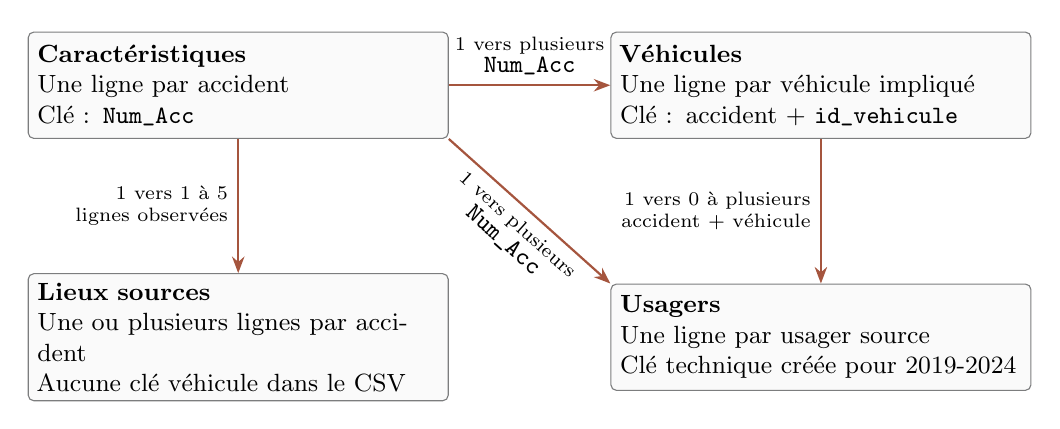
\begin{tikzpicture}[box/.style={draw=anthracite!60,rounded corners=2pt,fill=black!2,text width=5.1cm,minimum height=1.35cm,align=left,font=\small},
  edge/.style={-{Stealth[length=2.1mm]},thick,draw=terreCuite},every edge quotes/.style={font=\scriptsize}]
\node[box] (c) at (-3.7,0) {\textbf{Caractéristiques}\\Une ligne par accident\\Clé : \code{Num_Acc}};
\node[box] (v) at (3.7,0) {\textbf{Véhicules}\\Une ligne par véhicule impliqué\\Clé : accident + \code{id_vehicule}};
\node[box] (l) at (-3.7,-3.2) {\textbf{Lieux sources}\\Une ou plusieurs lignes par accident\\Aucune clé véhicule dans le CSV};
\node[box] (u) at (3.7,-3.2) {\textbf{Usagers}\\Une ligne par usager source\\Clé technique créée pour 2019-2024};
\draw[edge] (c.east) -- node[above,font=\scriptsize,align=center]{1 vers plusieurs\\\code{Num_Acc}} (v.west);
\draw[edge] (c.south) -- node[left,font=\scriptsize,align=right]{1 vers 1 à 5\\lignes observées} (l.north);
\draw[edge] (v.south) -- node[left,font=\scriptsize,align=right]{1 vers 0 à plusieurs\\accident + véhicule} (u.north);
\draw[edge] (c.south east) -- node[below,sloped,font=\scriptsize,align=center]{1 vers plusieurs\\\code{Num_Acc}} (u.north west);
\end{tikzpicture}
\caption{Relations contrôlées entre les tables sources. Les cardinalités décrivent les fichiers examinés ; elles sont vérifiées avant chaque jointure.}
\label{fig:relations}
\sourcecalcul{schéma du projet, à partir des notebooks 01 et 02}
\end{figure}

\section{Dimensions et différences de schéma}
\begin{table}[htbp]\centering\small
\caption{Nombre de lignes dans les sources complètes.}\label{tab:dimensions}
\begin{tabularx}{\textwidth}{@{}lLLLL@{}}\toprule
Année & Caractéristiques & Lieux & Véhicules & Usagers\\\midrule
2019 & 58\,840 & 58\,840 & 100\,710 & 132\,977\\
2020 & 47\,744 & 47\,744 & 81\,066 & 105\,295\\
2021 & 56\,518 & 56\,518 & 97\,315 & 129\,248\\
2022 & 55\,302 & 55\,302 & 94\,493 & 126\,662\\
2023 & 54\,822 & 70\,860 & 93\,585 & 125\,789\\
2024 & 54\,402 & 70\,248 & 92\,678 & 125\,187\\\bottomrule
\end{tabularx}
\sourcecalcul{notebook 02 ; nombre de lignes et non nombre de personnes pour toutes les colonnes}
\end{table}

Les caractéristiques comportent 15 colonnes, les lieux 18 et les véhicules 11. Les
usagers passent de 15 à 16 colonnes en 2021 avec l'apparition de \code{id_usager}.
En 2022, la clé des caractéristiques est nommée \code{Accident_Id}. Une concaténation
sans harmonisation ferait donc apparaître deux colonnes pour un même rôle.

Les espaces, dont des espaces insécables internes, concernent les identifiants de
véhicule et d'usager. La préparation les retirera dans toutes les tables liées.
Le contrôle vérifie qu'aucune valeur normalisée ne réunit plusieurs écritures brutes
distinctes dans une même colonne~: aucune collision n'est détectée.

\section{Clés, couverture et répétitions}
La clé accident est complète et unique dans les caractéristiques. La clé
\code{Num_Acc} + \code{id_vehicule} est unique dans les véhicules. Les identifiants
d'usager sont complets et uniques lorsqu'ils existent. Les ensembles d'accidents
des quatre tables sont identiques chaque année et chaque usager retrouve son véhicule.
Ces contrôles portent sur les identifiants eux-mêmes, pas seulement sur des effectifs
égaux.

La relation inverse est différente~: certains véhicules n'ont pas d'usager associé.
Sur les sources complètes, les nombres sont respectivement 2\,040, 1\,899, 6, 0, 40 et
24 entre 2019 et 2024. Le PDF explique les 24 cas de 2024 par des conducteurs en fuite
non créés dans la table des usagers~\cite{doc-onisr}. Cette explication ne doit pas être
étendue automatiquement à tous les écarts des autres années. Aucun usager ni aucune
gravité ne sont inventés pour compléter ces véhicules.

En 2019 et 2020, 101 et 63 lignes d'usagers supplémentaires sont identiques sur tous
leurs attributs sources. Sans identifiant individuel, ce constat ne prouve pas un
double enregistrement~: deux passagers peuvent avoir les mêmes caractéristiques.
Les lignes sont donc conservées et identifiées par leur rang source.

\section{Pourquoi les lieux demandent un traitement particulier}
Jusqu'en 2022, chaque accident possède une ligne de lieux. En 2023, 15\,870 accidents
ont plusieurs lignes, contre 15\,645 en 2024, soit respectivement 28,95\,\% et 28,76\,\%
des accidents des sources complètes. Le maximum observé est de cinq lignes. Certains
attributs varient et ces lignes ne sont donc pas de simples copies exactes.

L'accident \code{202400000005} illustre le problème. Quatre usagers sont associés à
deux lignes de lieux portant le même nom de voie, mais avec des limitations de 50 et
70 km/h et des profils de route différents. Une jointure brute sur \code{Num_Acc}
produirait huit lignes. La moyenne de 60 km/h, ou le choix de la première ligne,
n'aurait pas de justification comme limitation du lieu de chaque usager.

Dans sa réponse du 12 décembre 2024 à la discussion «~lieux-2023~», l'ONISR explique
que plusieurs lieux peuvent être décrits aux intersections, en lien avec les véhicules
concernés~\cite{discussion-lieux}. Les CSV reçus ne fournissent toutefois aucune clé
véhicule dans \code{lieux}. Le projet retiendra donc des informations communes au
niveau de l'accident. Cette explication ne démontre pas pourquoi la représentation
multiple apparaît à partir de 2023 dans ces exports.

\section{Codes, informations inconnues et plausibilité}
Le sens d'un code dépend de sa variable. \code{trajet = 0} désigne une information
non renseignée, alors que \code{secu1 = 0} signifie aucun équipement et
\code{vosp = 0} sans objet. Un remplacement global des zéros détruirait ces distinctions.
Certains codes observés sont absents de la rubrique du PDF, notamment 7 et 8 dans
\code{actp}. Ils sont signalés sans leur attribuer un sens supposé.

Les sources complètes contiennent 419 gravités inconnues~: 60 en 2021, 241 en 2022 et
118 en 2023. L'audit relève aussi 191 âges approximatifs supérieurs à 110 ans, issus
des naissances 1900 ou 1901 en 2019-2020. Des naissances manquantes apparaissent à partir
de 2021. Le PDF signale l'ajout d'usagers en fuite depuis 2021, avec des informations
parfois manquantes~\cite{doc-onisr}. Cette évolution constitue un contexte de collecte~;
elle ne permet pas d'identifier la cause de chaque valeur absente.

Les dates, heures et coordonnées passent les contrôles élémentaires appliqués~:
interprétation, concordance d'année et limites mondiales. Cela ne garantit pas que la
position GPS correspond au lieu réel. Le contrôle des communes métropolitaines révèle
trois discordances avec le département en 2019 et un code \code{N/C} en 2022. Sans
référentiel historique ni vérification complémentaire, l'audit ne choisit pas lequel
des deux renseignements corriger.

\FloatBarrier
\bilan{Les six années peuvent être réunies après harmonisation. Les risques principaux
concernent la multiplication des usagers par les lieux, la confusion entre codes
spéciaux et valeurs ordinaires, et une suppression injustifiée d'observations similaires.
Le chapitre suivant transforme ces constats en règles vérifiables.}

\chapter{Construction d'une table d'analyse fiable}
\label{chap:preparation}

Le notebook 03 repart des 24 CSV et construit une table métropolitaine par usager.
L'ordre des opérations est important~: les clés sont harmonisées, le périmètre est
sélectionné, les champs sont préparés et les lieux sont résumés avant toute jointure
finale. Les fichiers bruts ne sont pas modifiés.

\section{Lecture et conservation de la provenance}
Toutes les colonnes sont d'abord lues comme du texte, sans conversion automatique de
chaînes telles que \code{N/A} en valeurs manquantes. Une convention de lecture identique
évite de traiter différemment deux années avant même d'avoir défini les règles.

Chaque enregistrement reçoit son rang source et le chemin du CSV dont il provient.
Ce rang commence à 1 après l'en-tête~; il désigne un enregistrement CSV et pas forcément
une ligne physique si un champ contient un retour à la ligne. Le manifeste conserve
la taille, les dimensions et l'empreinte SHA-256 des 24 entrées. Les empreintes sont
revérifiées avant export pour détecter un changement pendant l'exécution.

L'identifiant \code{id_observation} combine l'année et le rang de l'usager, par exemple
\code{2024_usager_000011}. Il est créé pour toutes les années, y compris celles disposant
d'un identifiant officiel. Il reste stable pour une même version et un même ordre du
fichier source. Les usagers aux attributs identiques conservent des identifiants différents.

\section{Harmonisation et sélection géographique}
La clé \code{Accident_Id} de 2022 est renommée \code{Num_Acc}. Les espaces, y compris
internes et insécables, sont retirés des identifiants dans toutes les tables concernées.
Les clés et les collisions sont contrôlées avant de poursuivre. Le passage d'un code
de département comme 1 à 01 est explicite~; les codes 2A et 2B restent distincts.

La métropole est sélectionnée par une liste de 96 codes départementaux~: 01 à 95 hors
ancien code 20, auxquels s'ajoutent 2A et 2B. Le filtre repose sur le département déclaré
de l'accident, puis conserve les lieux, véhicules et usagers liés à ces accidents.
Un code inattendu provoquerait un arrêt pour examen, au lieu d'être silencieusement exclu.

Les codes commune sont aussi contrôlés. Un format non interprétable devient manquant
dans la colonne préparée, avec la valeur brute conservée. Une commune de format valide
dont le préfixe diffère du département est maintenue avec une alerte. Les quatre
accidents concernés par ces contrôles représentent six lignes d'usagers après jointure~:
le comptage d'une anomalie doit donc toujours préciser son unité.

Le tableau~\ref{tab:population-preparee} décrit le passage de 745\,158 usagers des sources
complètes à 702\,823 usagers métropolitains. Les 42\,335 lignes hors périmètre ne sont
pas des suppressions motivées par la gravité ou la qualité des variables.
\begin{table}[htbp]
\centering\small
\renewcommand{\arraystretch}{1.18}
\caption{Passage des sources complètes à la table métropolitaine.}\label{tab:population-preparee}
\begin{tabularx}{\textwidth}{@{}l>{\raggedleft\arraybackslash}X>{\raggedleft\arraybackslash}X>{\raggedleft\arraybackslash}X>{\raggedleft\arraybackslash}X@{}}
\toprule
Année & Usagers sources & Usagers retenus & Accidents retenus & Gravités inconnues retenues \\
\midrule
2019 & 132\,977 & 126\,352 & 56\,016 & 0 \\
2020 & 105\,295 & 99\,169 & 45\,121 & 0 \\
2021 & 129\,248 & 122\,189 & 53\,540 & 54 \\
2022 & 126\,662 & 119\,638 & 52\,380 & 215 \\
2023 & 125\,789 & 118\,197 & 51\,641 & 96 \\
2024 & 125\,187 & 117\,278 & 51\,058 & 0 \\
\textbf{Total} & 745\,158 & 702\,823 & 309\,756 & 365 \\
\bottomrule
\end{tabularx}
\sourcecalcul{notebook 03, bilan des effectifs}
\end{table}


\section{Règles pour les codes et les mesures}
Les colonnes catégorielles préparées contiennent un code documenté et interprétable,
ou une valeur manquante. Les variantes d'écriture telles que \code{1.0} sont ramenées
à \code{1}, mais le résultat reste du texte. Les lettres présentes dans certaines
rubriques sont préservées lorsque leur sens est documenté.

\begin{table}[htbp]\centering\small\renewcommand{\arraystretch}{1.2}
\caption{Exemples de règles appliquées aux valeurs particulières.}\label{tab:codes}
\begin{tabularx}{\textwidth}{@{}LLL@{}}\toprule
Situation & Interprétation & Traitement\\\midrule
\code{trajet = 0} & Non renseigné & Valeur préparée manquante.\\
\code{secu1 = 0} & Aucun équipement & Modalité conservée.\\
\code{vosp = 0} & Sans objet & Modalité conservée.\\
\code{actp = 0} & Non renseigné ou sans objet & Modalité mixte conservée, sans précision inventée.\\
Code non décrit, par exemple \code{actp = 7} & Sens non établi par la rubrique utilisée & Valeur préparée manquante, code source accessible.\\
\code{grav = -1} & Gravité inexploitable & Cible manquante, usager conservé.\\\bottomrule
\end{tabularx}
\sourcecalcul{règles du notebook 03, fondées sur la documentation et les valeurs observées}
\end{table}

Les codes \code{-1} sont laissés manquants~; lorsqu'ils ne figurent pas dans la liste
documentée d'un champ, ils sont aussi signalés comme non documentés dans le bilan.
Les colonnes brutes ou les CSV d'origine permettent de retrouver l'information initiale.
Les motifs de nettoyage sont comptés par variable et par table. Ils ne doivent pas être
additionnés pour produire un nombre de personnes~: une même ligne peut présenter
plusieurs difficultés et certaines tables décrivent des véhicules ou des lieux.

Le nombre de voies \code{nbv} et la vitesse maximale autorisée \code{vma} sont convertis
en mesures numériques. Une valeur vide, non numérique ou non positive devient manquante.
Un nombre de voies non entier est également inexploitable. Les autres valeurs positives
sont conservées. Les \code{vma} supérieures à 130 sont signalées pour examen, sans
correction supposée de 500 en 50. L'alerte porte sur 202 usagers associés à un accident
dont au moins un lieu dépasse ce seuil. Elle ne désigne ni 202 accidents ni une vitesse
réelle de véhicule~: \code{vma} est une limitation autorisée.

\section{Résumer les lieux sans inventer un lieu individuel}
Le résumé est construit séparément pour chaque variable au niveau de l'accident.
S'il reste une seule valeur connue distincte, elle est conservée. S'il existe plusieurs
valeurs connues, la valeur résumée est manquante et un indicateur signale le désaccord.
L'information partielle est un second indicateur, activé lorsqu'une valeur connue
coexiste avec une information inexploitable.

\begin{table}[htbp]\centering\small
\caption{Règle de résumé illustrée avec une limitation de vitesse.}\label{tab:consensus}
\begin{tabularx}{\textwidth}{@{}LLLL@{}}\toprule
Valeurs préparées & Résumé & Désaccord & Partielle\\\midrule
50, 50 & 50 & Non & Non\\
50, manquante & 50 & Non & Oui\\
50, 70 & Manquante & Oui & Non\\
50, 70, manquante & Manquante & Oui & Oui\\
Toutes manquantes & Manquante & Non & Non\\\bottomrule
\end{tabularx}
\sourcecalcul{convention du notebook 03 ; les indicateurs sont distincts}
\end{table}

Les champs résumés portent le préfixe \code{lieu_}. La règle est indépendante de l'ordre
des lignes et ne change pas si une répétition exacte est retirée. Pour l'accident
\code{202400000005}, la limitation résumée devient manquante avec désaccord, et les quatre
usagers restent quatre. En métropole, \code{vma} présente un désaccord entre valeurs
connues pour 1\,675 accidents en 2023 et 1\,875 en 2024. Ces nombres diffèrent des
variations brutes de l'audit, qui comptaient aussi les oppositions entre connu et inconnu.

Ce résumé est un compromis conservateur, pas une reconstitution du trajet de chaque
usager. Les lieux sources sont exportés séparément. Le nombre de lignes et les indicateurs
de désaccord servent d'abord à l'audit~; leur forte évolution entre années devra être
examinée avant tout usage prédictif.

\section{Âge, dates, coordonnées et cible}
L'âge approximatif est la différence entre l'année de l'accident et l'année de naissance.
L'anniversaire étant inconnu, il peut différer d'un an de l'âge exact. Les naissances
absentes, non interprétables ou non entières restent distinctes des âges hors intervalle.
La convention retenue conserve un âge préparé de 0 à 110 ans. Au-delà, l'âge devient
manquant, mais l'usager, l'estimation brute et l'indicateur d'alerte sont conservés.
Ce seuil est un outil de contrôle, pas une borne biologique démontrée.

Les 191 âges suspects des sources complètes deviennent 172 en métropole, dont 162 en
2019 et 10 en 2020. Le tableau~\ref{tab:qualite-preparee} présente les âges manquants
après traitement. Aucun âge n'est remplacé ici par une moyenne.
\begin{table}[htbp]
\centering\small
\renewcommand{\arraystretch}{1.18}
\caption{Quelques indicateurs de qualité dans le périmètre métropolitain.}\label{tab:qualite-preparee}
\begin{tabularx}{\textwidth}{@{}lLLL@{}}
\toprule
Année & Âges suspects & Âges manquants après traitement & Véhicules sans usager \\
\midrule
2019 & 162 & 162 & 1\,972 \\
2020 & 10 & 10 & 1\,838 \\
2021 & 0 & 2\,914 & 6 \\
2022 & 0 & 2\,732 & 0 \\
2023 & 0 & 2\,446 & 28 \\
2024 & 0 & 2\,419 & 23 \\
\bottomrule
\end{tabularx}
\sourcecalcul{notebook 03 ; les trois colonnes ne portent pas toutes sur la même unité}
\end{table}


Les dates sont converties et doivent correspondre à l'année du dossier~; les heures
doivent être interprétables. Des variables de mois, de jour de semaine et d'heure sont
créées. Les coordonnées utilisent un séparateur décimal harmonisé et un contrôle des
limites mondiales. Ces vérifications ne valident pas leur exactitude géographique.

La cible vaut 1 pour \code{grav} dans \{2,3\}, 0 pour \{1,4\}, et reste manquante sinon.
Les quatre catégories préparées et la gravité source restent accessibles. Les 419 gravités
inconnues des sources deviennent 365 en métropole~; la différence de 54 provient du
périmètre géographique. Ces 365 usagers sont conservés dans la table, mais ne devront
pas participer à un ajustement ou à une évaluation supervisés.

\section{Jointures et contrôles de conservation}
Les usagers constituent la table de départ. Le véhicule est ajouté sur
\code{Num_Acc} + \code{id_vehicule}, puis les caractéristiques et le résumé des lieux sur
\code{Num_Acc}. Chaque table de droite doit être unique sur sa clé. La validation
\code{many_to_one} interdit une multiplication des observations.

Avant et après chaque jointure, le programme compare l'effectif et l'ensemble des
\code{id_observation}. Il contrôle aussi les correspondances manquantes et l'accord des
deux versions de \code{num_veh}. Les 18 jointures annuelles conservent exactement leurs
usagers, sans correspondance manquante ni contradiction de numéro de véhicule.

Les champs propres aux piétons ne seront pas interprétés comme des comportements
piétons chez les autres usagers. Les trois équipements \code{secu1}, \code{secu2} et
\code{secu3} restent séparés~: aucun indicateur unique de protection n'est fabriqué
sans examiner leur contexte.

\section{Résultat, exports et relecture}
La table finale comporte \textbf{702\,823 lignes et 119 colonnes}, pour 309\,756 accidents.
Elle contient 702\,458 cibles connues et 365 inconnues. Aucun usager du périmètre n'a
été supprimé pour son âge, sa cible inconnue ou une variable explicative manquante.
Les 119 colonnes comprennent des identifiants, des valeurs sources, de la provenance
et des indicateurs de qualité~: elles ne forment pas une liste de 119 prédicteurs validés.

Deux CSV compressés sont produits~: la table des usagers et les lieux sources. Des JSON
décrivent les règles, les types, les rôles des colonnes et les empreintes. Six CSV de
bilan détaillent les effectifs, la géographie, les identifiants, les jointures, le
nettoyage et les lieux. L'annexe~\ref{ann:reproduction} en donne l'organisation.

Le CSV ne conserve pas les types Python. Le marqueur réservé
\code{__BAAC_MANQUANT__} distingue une valeur préparée manquante d'une chaîne vide
conservée dans un champ brut. Son absence dans les valeurs sources est vérifiée.
Une relecture par blocs applique le schéma, le marqueur et les conversions de date,
puis compare les 702\,823 lignes, toutes les colonnes, leurs valeurs et leurs types.

\FloatBarrier
\bilan{La table est exploitable sans confondre absence d'information et classe négative.
Les contrôles garantissent la conservation et la traçabilité des observations dans
les fichiers examinés. Ils ne corrigent pas les biais de collecte ni toutes les erreurs
de renseignement possibles.}

\chapter{Analyse exploratoire de la population et de la gravité}
\label{chap:exploration}

Une fois la table préparée, le notebook 04 décrit les usagers et les différences de
gravité. Chaque graphique répond à une question et les tableaux conservent les effectifs
qui permettent d'interpréter les pourcentages. Les résultats de ce chapitre sont
descriptifs~; leurs intervalles de variabilité seront examinés au chapitre suivant.

\section{Population analysée et dénominateurs}
Le chargement parcourt le fichier préparé par blocs et conserve uniquement 2019-2022.
Ces années correspondent à la période d'apprentissage. Les comparaisons de gravité de
ce chapitre ne portent pas sur 2023 ou 2024, même si ces années ont participé aux audits.

La population comprend 467\,348 usagers et 207\,057 accidents. La gravité est connue
pour 467\,079 usagers et inconnue pour 269. On compte 83\,081 décès ou hospitalisations,
soit 17,79\,\% des gravités connues. Ce pourcentage est une proportion par usager~;
un accident impliquant plusieurs personnes contribue plusieurs observations.

Pour chaque groupe, le dénominateur est le nombre d'usagers de ce groupe dont la cible
est connue. Par exemple, un cas positif, un cas négatif et une gravité inconnue donnent
une proportion de $1/2$, et non de $1/3$. Un groupe sans gravité connue ne reçoit pas
une proportion de zéro~: cette proportion n'est pas définie. Les effectifs de cibles
inconnues restent présentés dans les sorties du notebook.

\section{Effectifs et profils des usagers}
\subsection{Les volumes enregistrés varient selon l'année}
Le tableau~\ref{tab:population-train} sépare les effectifs d'usagers et d'accidents.
La proportion annuelle se calcule sur les cibles connues de l'année. La proportion
globale résulte de la somme des numérateurs et dénominateurs~; elle n'est pas la moyenne
non pondérée des quatre pourcentages annuels.
\begin{table}[htbp]
\centering\small
\renewcommand{\arraystretch}{1.18}
\caption{Population et proportion de décès ou hospitalisations, 2019-2022.}\label{tab:population-train}
\begin{tabularx}{\textwidth}{@{}lLLLLL@{}}
\toprule
Année & Usagers & Accidents & Gravités connues & Cas positifs & Proportion (\%) \\
\midrule
2019 & 126\,352 & 56\,016 & 126\,352 & 22\,853 & 18,09 \\
2020 & 99\,169 & 45\,121 & 99\,169 & 18\,141 & 18,29 \\
2021 & 122\,189 & 53\,540 & 122\,135 & 20\,796 & 17,03 \\
2022 & 119\,638 & 52\,380 & 119\,423 & 21\,291 & 17,83 \\
\bottomrule
\end{tabularx}
\sourcecalcul{notebook 04 ; dénominateur : gravités connues de chaque année}
\end{table}

\figurerapport{04_01_effectifs_annuels.png}{Évolution des usagers enregistrés et des accidents distincts. Les deux unités utilisent des axes séparés.}{fig:volumes}

La baisse des volumes en 2020 est visible dans les deux unités. Ces courbes ne séparent
pas les effets de l'exposition routière, des pratiques d'enregistrement et des autres
changements de contexte. Les seules données représentées ne suffisent pas à attribuer
la variation à une cause précise ni à en déduire une évolution du risque par trajet.
\FloatBarrier

\subsection{Âge approximatif et catégorie d'usager}
Parmi les 461\,530 âges préparés connus, la médiane est de 35 ans, les quartiles de
23 et 52 ans et la moyenne d'environ 38,5 ans. L'histogramme utilise des classes de
cinq ans. Il décrit la distribution des personnes enregistrées dont l'âge est connu,
sans représenter la population générale française.
\figurerapport[0.90]{04_02_distribution_age.png}{Distribution des âges approximatifs connus. Les 5 818 âges manquants sont comptés séparément.}{fig:ages}

Les conducteurs représentent environ 74,5\,\% des usagers, les passagers 17,7\,\% et
les piétons 7,8\,\%. Ces parts décrivent la composition des accidents enregistrés.
Une catégorie plus nombreuse n'est pas nécessairement celle dont la proportion de
décès ou d'hospitalisations est la plus élevée.
\figurerapport[0.88]{04_03_categories_usagers.png}{Répartition des catégories d'usagers dans la population analysée.}{fig:catu-pop}
\FloatBarrier

\section{Répartition des catégories de gravité}
Les quatre modalités sont conservées pour distinguer ce que le regroupement binaire
réunit. On observe 196\,270 indemnes, 11\,996 tués, 71\,085 blessés hospitalisés et
187\,728 blessés légers, auxquels s'ajoutent les 269 gravités inconnues.
Les pourcentages de la figure~\ref{fig:gravite} portent sur tous les usagers, y compris
les inconnus~; le taux de la cible binaire porte, lui, sur les seules gravités connues.
\figurerapport[0.90]{04_04_repartition_gravite.png}{Répartition des quatre modalités originales et des gravités inconnues, 2019-2022.}{fig:gravite}

Les décès seuls représentent 2,57\,\% des gravités connues, contre 17,79\,\% pour décès
ou hospitalisation. Cette différence de fréquence justifie de lire les deux définitions
séparément. Une méthode prédictive sera comparée à une référence simple et évaluée
au-delà de sa seule proportion globale de réponses correctes.
\FloatBarrier

\section{Comparer les proportions selon les caractéristiques}
\subsection{Âge}
La proportion est de 20,40\,\% chez les 0-17 ans, descend à 13,91\,\% chez les 35-44 ans,
puis atteint 33,26\,\% chez les 75 ans ou plus. Cette forme ne correspond pas à une
progression linéaire unique de la proportion avec l'âge. Les groupes ont aussi des
compositions différentes en matière de déplacement et de contexte.
\figurerapport{04_05_gravite_selon_age.png}{Décès ou hospitalisation selon la tranche d'âge. $n$ désigne les gravités connues ; le trait représente la proportion globale de 17,8\,\%.}{fig:age-gravite}
\begin{table}[htbp]
\centering\small
\renewcommand{\arraystretch}{1.18}
\caption{Gravité selon l'âge, 2019-2022.}\label{tab:gravite-age}
\begin{tabularx}{\textwidth}{@{}>{\hsize=1.65\hsize\linewidth=\hsize}L>{\hsize=.8\hsize\linewidth=\hsize}L>{\hsize=.75\hsize\linewidth=\hsize}L>{\hsize=.8\hsize\linewidth=\hsize}L@{}}
\toprule
Groupe & Gravités connues & Cas positifs & Proportion (\%) \\
\midrule
0-17 ans & 41\,349 & 8\,437 & 20,40 \\
18-24 ans & 87\,449 & 15\,629 & 17,87 \\
25-34 ans & 97\,065 & 13\,814 & 14,23 \\
35-44 ans & 73\,461 & 10\,222 & 13,91 \\
45-54 ans & 64\,377 & 10\,560 & 16,40 \\
55-64 ans & 47\,758 & 9\,752 & 20,42 \\
65-74 ans & 27\,652 & 7\,200 & 26,04 \\
75 ans ou plus & 22\,418 & 7\,457 & 33,26 \\
Âge inconnu & 5\,550 & 10 & 0,18 \\
\bottomrule
\end{tabularx}
\sourcecalcul{notebook 04 ; les gravités inconnues sont exclues du dénominateur}
\end{table}


La tranche 35-44 ans est retenue comme référence descriptive pour la comparaison
avec les 75 ans ou plus. Ce choix est intervenu après l'exploration~: il ne s'agit pas
d'un contraste confirmé à partir d'une hypothèse annoncée avant observation.
\FloatBarrier

\subsection{Catégorie d'usager}
Les proportions sont proches pour les conducteurs et les passagers, autour de 16\,\%,
et plus élevées pour les piétons, à 32,60\,\%. Le tableau~\ref{tab:gravite-categorie}
montre que cette différence ne s'explique pas par la simple taille des groupes~:
les piétons sont moins nombreux mais leur proportion positive est plus forte.
\figurerapport{04_06_gravite_selon_categorie.png}{Proportions selon la catégorie d'usager ; les effectifs indiqués excluent les gravités inconnues.}{fig:catu-gravite}
\begin{table}[htbp]
\centering\small
\renewcommand{\arraystretch}{1.18}
\caption{Gravité selon la catégorie d'usager, 2019-2022.}\label{tab:gravite-categorie}
\begin{tabularx}{\textwidth}{@{}>{\hsize=1.65\hsize\linewidth=\hsize}L>{\hsize=.8\hsize\linewidth=\hsize}L>{\hsize=.75\hsize\linewidth=\hsize}L>{\hsize=.8\hsize\linewidth=\hsize}L@{}}
\toprule
Groupe & Gravités connues & Cas positifs & Proportion (\%) \\
\midrule
Conducteur & 347\,962 & 57\,674 & 16,57 \\
Passager & 82\,591 & 13\,498 & 16,34 \\
Piéton & 36\,526 & 11\,909 & 32,60 \\
\bottomrule
\end{tabularx}
\sourcecalcul{notebook 04 ; les gravités inconnues sont exclues du dénominateur}
\end{table}


Cette comparaison n'isole pas un effet causal du statut de piéton. Elle peut refléter
des différences d'âge, de contexte et de véhicules impliqués. Pour les piétons, le
véhicule associé est celui qui les a heurtés~; une future analyse par catégorie de
véhicule devra conserver cette distinction.
\FloatBarrier

\subsection{Lumière}
La proportion est de 16,94\,\% en plein jour et de 28,79\,\% de nuit sans éclairage
public. Les autres modalités ont des niveaux différents~: 20,14\,\% à l'aube ou au
crépuscule, 19,58\,\% de nuit avec éclairage public éteint et 13,45\,\% avec éclairage
public allumé. Regrouper toutes les nuits masquerait ces différences.
\figurerapport{04_07_gravite_selon_lumiere.png}{Proportions selon la lumière. La modalité non renseignée figure dans le tableau, mais pas dans les barres des modalités connues.}{fig:lum-gravite}
\begin{table}[htbp]
\centering\small
\renewcommand{\arraystretch}{1.18}
\caption{Gravité selon la lumière, 2019-2022.}\label{tab:gravite-lumiere}
\begin{tabularx}{\textwidth}{@{}>{\hsize=1.65\hsize\linewidth=\hsize}L>{\hsize=.8\hsize\linewidth=\hsize}L>{\hsize=.75\hsize\linewidth=\hsize}L>{\hsize=.8\hsize\linewidth=\hsize}L@{}}
\toprule
Groupe & Gravités connues & Cas positifs & Proportion (\%) \\
\midrule
Plein jour & 316\,041 & 53\,546 & 16,94 \\
Crépuscule ou aube & 30\,196 & 6\,082 & 20,14 \\
Nuit sans éclairage public & 45\,404 & 13\,072 & 28,79 \\
Nuit, éclairage public éteint & 3\,872 & 758 & 19,58 \\
Nuit, éclairage public allumé & 71\,557 & 9\,622 & 13,45 \\
Non renseigné & 9 & 1 & 11,11 \\
\bottomrule
\end{tabularx}
\sourcecalcul{notebook 04 ; les gravités inconnues sont exclues du dénominateur}
\end{table}


La faible proportion observée lorsque l'éclairage public est allumé ne mesure pas
l'effet propre d'un éclairage~: les types de routes, l'agglomération et les profils
d'usagers peuvent différer. La modalité non renseignée ne compte que neuf gravités
connues~; son pourcentage ne justifie pas une interprétation substantielle.
\FloatBarrier

\subsection{Agglomération}
La proportion atteint 25,90\,\% hors agglomération, contre 12,89\,\% en agglomération.
Les effectifs restent élevés dans les deux groupes. Cette différence décrit le contexte
des accidents enregistrés~; elle ne fournit ni un risque par kilomètre ni la mesure
d'un effet isolé de la vitesse, qui n'est pas directement observée par \code{vma}.
\figurerapport{04_08_gravite_selon_agglomeration.png}{Proportions de décès ou hospitalisations en et hors agglomération, 2019-2022.}{fig:agg-gravite}
\begin{table}[htbp]
\centering\small
\renewcommand{\arraystretch}{1.18}
\caption{Gravité selon l'agglomération, 2019-2022.}\label{tab:gravite-agglomeration}
\begin{tabularx}{\textwidth}{@{}>{\hsize=1.65\hsize\linewidth=\hsize}L>{\hsize=.8\hsize\linewidth=\hsize}L>{\hsize=.75\hsize\linewidth=\hsize}L>{\hsize=.8\hsize\linewidth=\hsize}L@{}}
\toprule
Groupe & Gravités connues & Cas positifs & Proportion (\%) \\
\midrule
Hors agglomération & 175\,858 & 45\,555 & 25,90 \\
En agglomération & 291\,221 & 37\,526 & 12,89 \\
\bottomrule
\end{tabularx}
\sourcecalcul{notebook 04 ; les gravités inconnues sont exclues du dénominateur}
\end{table}

\FloatBarrier

\section{Valeurs manquantes et lecture annuelle}
Les 5\,818 âges manquants comprennent 5\,550 usagers à gravité connue, dont seulement
10 décès ou hospitalisations, soit 0,18\,\%. Les 268 autres ont une gravité inconnue.
L'absence d'âge est donc associée à une répartition particulière de la gravité. Ce
constat invite à examiner le mécanisme de collecte et la stabilité temporelle d'un
éventuel indicateur d'âge manquant. Il ne permet pas d'affirmer que tous ces usagers
sont en fuite ni de les supprimer par principe.

Les tableaux annuels du notebook reprennent les comparaisons par catégorie d'usager
et agglomération. Leur orientation demeure la même chaque année, mais leurs niveaux
varient. Le chapitre suivant prolonge cette vérification pour les quatre contrastes.
Une persistance annuelle ne constitue pas un ajustement sur les autres caractéristiques.

\section{Ce que l'exploration permet de retenir}
L'âge, la catégorie d'usager, la lumière et l'agglomération présentent des écarts
descriptifs qui méritent d'être quantifiés. Les comparaisons gardent les valeurs
manquantes visibles et précisent leurs dénominateurs. Elles ne recherchent pas toutes
les relations possibles entre les 119 colonnes.

Les codes des catégories ne sont pas traités comme des nombres ordonnés. Les résultats
présentés sont des distributions et des proportions conditionnelles~; aucune matrice
de corrélations de Pearson sur les codes bruts n'est utilisée comme preuve d'association.
Des analyses sur d'autres variables ou avec ajustement simultané resteraient des
travaux supplémentaires, à définir en fonction d'une question précise.

\bilan{L'exploration fournit un portrait de la population et quatre contrastes motivés.
Elle établit leur sens et leur ampleur descriptive. Elle ne mesure pas encore leur
variabilité sous un processus de répétition et ne sépare pas les contributions des
différentes caractéristiques.}

\chapter[Analyse statistique et probabiliste des écarts de gravité]{Analyse statistique et probabiliste\\des écarts de gravité}
\label{chap:statistiques}

Le notebook 05 prolonge l'exploration par des écarts absolus, des rapports de proportions
et des intervalles bootstrap. La question n'est pas seulement de savoir si deux
pourcentages diffèrent~: il faut préciser la quantité estimée, son dénominateur et le
processus de répétition auquel son intervalle se rapporte.

\section{Probabilités conditionnelles et variable de Bernoulli}
Pour un usager à gravité connue, $Y$ vaut 1 en cas de décès ou d'hospitalisation et 0
sinon. Pour un usager tiré au hasard dans la population définie, $Y$ est une variable
de Bernoulli de paramètre $p$, avec $E(Y)=p$ et $\operatorname{Var}(Y)=p(1-p)$.
Cette description marginale n'impose pas que les usagers d'un même accident soient
indépendants.

Notons $S$ le périmètre des usagers d'accidents corporels enregistrés en métropole en
2019-2022, avec gravité connue. Pour un groupe $G$, la quantité étudiée est
\begin{equation}
 p_G=P(Y=1\mid G,S),\qquad
 \widehat p_G=\frac{n_{G,1}}{n_{G,0}+n_{G,1}},
 \label{eq:proportion}
\end{equation}
où $n_{G,1}$ et $n_{G,0}$ sont les effectifs positifs et négatifs connus du groupe.
L'estimateur est pondéré par les usagers, pas par un poids égal attribué à chaque accident.

\section{Contrastes retenus et mesure de leur ampleur}
Quatre comparaisons sont fixées à partir de l'exploration~: 75 ans ou plus contre
35-44 ans, piétons contre conducteurs, nuit sans éclairage public contre plein jour,
et hors agglomération contre en agglomération. L'orientation A / R reste identique
dans les tableaux, les graphiques et les réplications.

Deux mesures sont complémentaires~:
\begin{equation}
 \Delta=100(p_A-p_R)\quad\text{en points de pourcentage},\qquad
 R_p=\frac{p_A}{p_R}\quad\text{sans unité}.
 \label{eq:contrastes}
\end{equation}
Un écart entre 32,6\,\% et 16,6\,\% représente environ 16 points de pourcentage et un
rapport de 1,97. Ce rapport est un rapport de proportions conditionnelles, pas un
rapport de risques d'accident par trajet, ni un rapport de cotes (\textit{odds ratio}).
Si la proportion de référence est nulle, le rapport reste indéfini.

Dans chaque contraste, A et R sont disjoints. En revanche, les groupes de dimensions
différentes se recoupent~: un piéton peut aussi avoir plus de 75 ans et être impliqué
hors agglomération. Les comptages des neuf groupes, ensemble inclus, ne doivent donc
pas être additionnés pour reconstruire la population.

\section{Quel sens donner à un intervalle ici~?}
Les proportions sont des descriptions exactes des enregistrements disponibles. BAAC
n'est pas un échantillon aléatoire simple de tous les déplacements. Les intervalles
ne sont donc pas une marge d'erreur garantie sur l'ensemble des accidents réels.

Le cadre retenu est une répétition hypothétique~: si des accidents comparables étaient
enregistrés à nouveau dans les mêmes années et avec des pratiques de collecte
comparables, quelle variabilité nos statistiques pourraient-elles présenter~? Les
accidents sont supposés approximativement indépendants au sein d'une année et leur
distribution empirique représente le processus envisagé. Les années sont fixes et
les personnes restent liées à l'intérieur de chaque accident.

Ce cadre ne modélise pas une dépendance spatiale ou temporelle supplémentaire entre
accidents. Il ne corrige ni la sous-déclaration, ni les erreurs de renseignement, ni
les gravités inconnues. La prudence d'interprétation reste nécessaire même avec un
grand effectif et un intervalle étroit.

\section{Bootstrap par accident, stratifié par année}
Le rééchantillonnage de groupes entiers et la sélection séparée dans les strates sont
des mécanismes décrits par le manuel \textit{bsample}~\cite{stata-bsample}. Notre choix
de l'accident comme groupe et de l'année comme strate répond à l'organisation de BAAC.
La référence décrit le mécanisme, sans valider à elle seule toutes ses hypothèses ici.

Un exemple fictif rend la règle concrète. Trois accidents A, B et C comportent
respectivement 2, 1 et 3 usagers, dont 1, 0 et 2 cas positifs. La proportion observée
est $3/6=50\,\%$. Un tirage A, A, C conserve les deux copies de A~: il comprend sept
usagers et quatre positifs, soit $4/7$. Le nombre de tirages d'accidents est inchangé,
mais le nombre d'usagers varie. Éliminer les tirages répétés ou conserver seulement
un usager par accident changerait la méthode.

Pour chaque réplication réelle, autant d'accidents que ceux observés en 2019 sont
tirés avec remise, puis l'opération est répétée séparément pour 2020, 2021 et 2022.
Les contributions sont regroupées pour calculer les proportions de la période.
Les 207\,057 accidents sont conservés dans la base de tirage, y compris ceux dont
la contribution est nulle pour un groupe donné ou pour les gravités connues.

L'implémentation utilise une matrice de comptages par accident~: pour chacun des neuf
groupes, elle stocke les gravités connues, les cas positifs principaux et les décès.
Les 27 colonnes suffisent aux statistiques calculées. La somme des comptages des
accidents tirés est équivalente à la copie de leurs usagers, avec leurs répétitions.
Cette équivalence a été vérifiée sur un exemple indépendant.

Le nombre de réplications est $B=2\,000$ et la graine est 20261016. Chaque année utilise
\code{numpy.default_rng} avec une initialisation fondée sur la graine et l'année.
Les mêmes tirages servent à tous les groupes et aux deux définitions de gravité~:
les liens entre personnes et entre statistiques sont ainsi conservés. Les intervalles
des écarts sont calculés sur les écarts répliqués, sans soustraire les bornes de deux
intervalles de proportions séparés.

\subsection{Construction des bornes percentiles}
Pour une statistique $T$, les réplications $T_1^*,\ldots,T_B^*$ donnent l'intervalle
percentile nominal à 95\,\%~\cite{nist-bootstrap}~:
\begin{equation}
 \left[q_{0,025}(T^*),\ q_{0,975}(T^*)\right].
 \label{eq:ic}
\end{equation}
Les quantiles utilisent une interpolation linéaire. Il s'agit d'une approximation
simple non corrigée du biais. Le niveau de 95\,\% concerne la procédure dans un cadre
de répétition~; il n'attribue pas une probabilité de 95\,\% à un paramètre fixé à
l'intérieur de l'intervalle déjà calculé.

Les intervalles sont marginaux, un par statistique, et ne garantissent pas une
couverture simultanée de toutes les comparaisons. Si une réplication rend une
statistique indéfinie, le programme signale le nombre de valeurs valides et laisse
l'intervalle manquant, sans écarter silencieusement cette réplication. Tous les
contrastes présentés disposent ici de 2\,000 valeurs valides.

\section{Résultats pour décès ou hospitalisation}
Le tableau~\ref{tab:deces_hospitalisation} et la figure~\ref{fig:forest-principal}
présentent les résultats regroupés. Les quatre écarts sont positifs et leurs
intervalles restent au-dessus de zéro dans le cadre de répétition retenu.
\begin{table}[htbp]
\centering\small
\renewcommand{\arraystretch}{1.18}
\caption{Écarts et rapports : décès ou hospitalisation, 2019-2022.}\label{tab:deces_hospitalisation}
\begin{tabular*}{\textwidth}{@{\extracolsep{\fill}}lrrrr@{}}
\toprule
Comparaison A / R & Écart (points) & IC à 95\% & Rapport & IC à 95\% \\
\midrule
75+ / 35-44 ans & 19,35 & [18,69 ; 20,04] & 2,39 & [2,33 ; 2,46] \\
Piétons / conducteurs & 16,03 & [15,52 ; 16,54] & 1,97 & [1,93 ; 2,00] \\
Nuit sans éclairage / jour & 11,85 & [11,35 ; 12,38] & 1,70 & [1,67 ; 1,73] \\
Hors / en agglomération & 13,02 & [12,76 ; 13,28] & 2,01 & [1,98 ; 2,04] \\
\bottomrule
\end{tabular*}
\sourcecalcul{notebook 05 ; intervalles percentiles marginaux, 2 000 réplications d'accidents stratifiées par année}
\end{table}

\figurerapport{05_01_contrastes_cible_principale.png}{Écarts en points et rapports de proportions pour la cible principale. Les références sont respectivement zéro et un.}{fig:forest-principal}

Pour les piétons, la proportion atteint 32,60\,\%, contre 16,57\,\% pour les conducteurs.
L'écart est de 16,03 points, avec un intervalle [15,52~; 16,54], et le rapport de 1,97,
avec un intervalle [1,93~; 2,00]. Pour l'âge, l'écart est plus grand, à 19,35 points,
mais il concerne deux tranches choisies après l'exploration. Les rapports de 1,70 pour
la lumière et 2,01 pour l'agglomération résument des différences brutes.

Ces résultats ne désignent pas quatre effets indépendants. Une partie de leurs écarts
peut refléter des compositions communes en âge, véhicule ou contexte. Le fait qu'un
intervalle exclue zéro ne transforme pas l'association en effet causal et ne résout
pas le caractère exploratoire de la sélection des comparaisons.
\FloatBarrier

\subsection{Distribution des réplications et stabilité numérique}
La figure~\ref{fig:hist-bootstrap} représente les 2\,000 écarts piétons-conducteurs.
Elle décrit une distribution de statistiques répliquées, et non une distribution de
blessures ou une population de 2\,000 usagers. Les traits encadrent les bornes percentiles.
\figurerapport[0.90]{05_02_distribution_bootstrap_pietons.png}{Distribution bootstrap de l'écart piétons-conducteurs. Chaque valeur résulte d'un nouveau tirage d'accidents dans les quatre années.}{fig:hist-bootstrap}

Les bornes calculées avec les 1\,000 premières réplications sont comparées à celles
des 2\,000 réplications, pour les écarts en points. La variation maximale est de
0,0350 point, soit environ 0,04 point de pourcentage. Ce contrôle indique une faible
sensibilité numérique sur cette exécution~; il ne prouve ni la couverture réelle
des intervalles ni la validité des hypothèses.
\begin{table}[htbp]
\centering\small
\renewcommand{\arraystretch}{1.18}
\caption{Variation maximale d'une borne d'écart entre 1 000 et 2 000 réplications.}\label{tab:stabilite}
\begin{tabularx}{\textwidth}{@{}LLL@{}}
\toprule
Comparaison & Cible principale (points) & Décès seuls (points) \\
\midrule
75+ / 35-44 ans & 0,0350 & 0,0307 \\
Piétons / conducteurs & 0,0118 & 0,0031 \\
Nuit sans éclairage / jour & 0,0161 & 0,0109 \\
Hors / en agglomération & 0,0048 & 0,0045 \\
\bottomrule
\end{tabularx}
\sourcecalcul{notebook 05 ; contrôle numérique sur une graine fixée}
\end{table}

\FloatBarrier

\clearpage
\section{Lecture annuelle et sensibilité aux décès seuls}
\subsection{Les différences gardent-elles le même sens chaque année~?}
Les comparaisons sont recalculées pour chaque année à partir des proportions et des
réplications propres à cette année. Les années elles-mêmes ne sont pas rééchantillonnées.
Les quatre écarts observés restent positifs en 2019, 2020, 2021 et 2022. L'écart d'âge
est cependant plus faible en 2021-2022 qu'en 2019-2020.
\figurerapport{05_03_contrastes_annuels.png}{Écarts annuels pour la cible principale. Les zones représentent des intervalles marginaux par année, sans couverture simultanée ni prévision d'une année future.}{fig:contrastes-annuels}

La répétition du sens des écarts renforce leur constat descriptif sur la période.
Elle ne sépare pas les contributions des autres variables et ne démontre pas un effet
du temps. Les bandes ne sont pas des intervalles de prévision pour 2023 ou 2024.
\FloatBarrier

\subsection{Changer l'événement : décès seuls}
La cible complémentaire vaut 1 pour les décès et 0 pour les trois autres modalités
connues. Les gravités inconnues restent exclues du dénominateur. Les mêmes 467\,079
usagers à gravité connue et les mêmes tirages sont donc utilisés. On compte
11\,996 décès, soit 2,57\,\%.
\begin{table}[htbp]
\centering\small
\renewcommand{\arraystretch}{1.18}
\caption{Écarts et rapports : décès seuls, 2019-2022.}\label{tab:deces_seul}
\begin{tabular*}{\textwidth}{@{\extracolsep{\fill}}lrrrr@{}}
\toprule
Comparaison A / R & Écart (points) & IC à 95\% & Rapport & IC à 95\% \\
\midrule
75+ / 35-44 ans & 6,44 & [6,06 ; 6,84] & 4,27 & [4,00 ; 4,61] \\
Piétons / conducteurs & 2,39 & [2,16 ; 2,63] & 1,98 & [1,88 ; 2,08] \\
Nuit sans éclairage / jour & 4,12 & [3,87 ; 4,37] & 2,87 & [2,74 ; 3,01] \\
Hors / en agglomération & 3,27 & [3,15 ; 3,38] & 3,44 & [3,30 ; 3,58] \\
\bottomrule
\end{tabular*}
\sourcecalcul{notebook 05 ; intervalles percentiles marginaux, 2 000 réplications d'accidents stratifiées par année}
\end{table}

\figurerapport{05_04_contrastes_deces_seuls.png}{Écarts et rapports pour les décès seuls. Une différence absolue plus faible peut coexister avec un rapport plus élevé.}{fig:forest-deces}
\FloatBarrier

Chez les 75 ans ou plus, la proportion de décès est de 8,41\,\%, contre 1,97\,\% chez
les 35-44 ans~: l'écart vaut 6,44 points et le rapport 4,27. Le rapport principal
était de 2,39. Les rapports pour la lumière et l'agglomération sont aussi plus élevés
avec les décès seuls, alors que celui des piétons reste proche de deux.

La définition de l'événement change donc la lecture quantitative. Cette analyse
permet d'examiner la sensibilité à l'hospitalisation~; elle ne justifie pas de choisir
une cible parce qu'elle produit un contraste plus spectaculaire.
\FloatBarrier

\clearpage
\section{Bilan de la première partie et limites}
La première partie a produit une table métropolitaine traçable, des contrôles de
jointure, un portrait des usagers et des comparaisons dont les dénominateurs sont
explicites. Les écarts observés selon l'âge, la catégorie d'usager, la lumière et
l'agglomération persistent dans la lecture annuelle de 2019-2022. Leur amplitude
dépend de la définition de la gravité.

Trois limites restent structurantes. Les accidents enregistrés ne représentent pas
tous les trajets ni nécessairement tous les accidents réels. L'hospitalisation et
les informations inconnues sont sensibles à la collecte. Enfin, les comparaisons
sont brutes et certaines caractéristiques se recoupent. Le bootstrap ne supprime
aucune de ces limites et n'intègre pas toutes les dépendances possibles entre accidents.

La seconde partie étudie plusieurs caractéristiques simultanément et évalue des
probabilités sur une année ultérieure, avec une référence constante et un protocole
temporel déclaré. La gravité et ses dérivés sont exclus des prédicteurs, les traitements
appris restent limités à l'apprentissage et les mécanismes de valeurs manquantes
font l'objet de diagnostics spécifiques.

\clearpage

\addtocontents{toc}{\protect\newpage}
\part{Modélisation probabiliste et évaluation prédictive}
\chapter{Construire une estimation probabiliste de la gravité}
\label{chap:protocole-ml}

Les analyses précédentes comparent les groupes séparément. Elles montrent des écarts,
mais ne disent pas comment plusieurs caractéristiques, considérées ensemble, permettent
d'estimer une issue individuelle. Le volet prédictif répond à cette seconde question.
Son résultat est une probabilité de décès ou d'hospitalisation parmi les usagers
d'accidents corporels enregistrés. Aucun scénario de prédiction avant un trajet n'est
défini dans cette étude.

\section{Ce que le modèle cherche à estimer}
Pour un usager décrit par $x$, la quantité estimée est
\[
  p(x)=\mathbb{P}(Y=1\mid X=x,\ \text{usager présent dans BAAC}).
\]
La cible $Y$ conserve la définition du chapitre~\ref{chap:cadrage}. Les gravités
inconnues sont exclues de l'ajustement et des scores, après comptage. Le modèle ne
distingue donc pas les décès des hospitalisations à l'intérieur de la classe positive.

La comparaison est volontairement limitée à une référence constante et à une
régression logistique. Cette dernière combine plusieurs caractéristiques, produit
directement des probabilités et permet une lecture des coefficients. Un modèle plus
complexe n'est pas nécessaire pour vérifier si ces informations apportent déjà un gain.
Ce choix limite aussi le nombre d'expériences utilisées pour sélectionner une solution.

\section{Séparer les années avant l'apprentissage}
L'apprentissage porte sur 2019-2022, la validation sur 2023 et le test final sur 2024.
La validation sert à choisir le réglage du modèle. Le test sert ensuite à mesurer les
performances de cette configuration sur une année ultérieure.
\begin{table}[htbp]
\centering\small
\renewcommand{\arraystretch}{1.18}
\caption{Populations utilisées pour la modélisation, après exclusion des gravités inconnues.}\label{tab:ml-population}
\begin{tabular*}{\textwidth}{@{\extracolsep{\fill}}lrrrr@{}}
\toprule
Période & Cibles connues & Exclues & Cas positifs & Part (\%) \\
\midrule
2019-2022 & 467\,079 & 269 & 83\,081 & 17,79 \\
2023 & 118\,101 & 96 & 21\,218 & 17,97 \\
2024 & 117\,278 & 0 & 21\,024 & 17,93 \\
\bottomrule
\end{tabular*}
\sourcecalcul{notebooks 06 et 07 ; les exclusions portent uniquement sur la cible inconnue}
\end{table}


Une séparation par année maintient tous les usagers d'un accident dans la même
partition. Elle évite qu'un conducteur soit utilisé pour apprendre tandis qu'un
passager du même accident servirait à évaluer le modèle. Elle conserve également les
changements entre millésimes dans l'évaluation.

L'année 2024 a toutefois été examinée lors des audits de structure. Ce test est donc
\textbf{rétrospectif et chronologique}, et non une expérience prospective sur un jeu
resté totalement inconnu. Ses scores n'ont pas servi à sélectionner les variables,
les valeurs de régularisation ou le seuil. Maintenant qu'ils sont consultés, cette
année ne peut plus être réutilisée comme un nouveau test vierge.

\section{Choisir des variables et rendre leur représentation explicite}
Onze variables sources sont retenues avant la comparaison des scores. Elles décrivent
l'usager, le véhicule associé et les circonstances de l'accident.

\begin{table}[htbp]\centering\small
\caption{Variables du premier modèle et représentation retenue.}\label{tab:variables-ml}
\renewcommand{\arraystretch}{1.17}
\begin{tabularx}{\textwidth}{@{}lLL@{}}\toprule
Famille & Variables sources & Représentation et précautions\\\midrule
Usager & \code{age_approx}, \code{sexe}, \code{catu} & Âge en huit tranches fixes ; sexe et catégorie comme modalités.\\
Véhicule & \code{catv} & Catégorie du véhicule associé ; véhicule heurtant pour un piéton.\\
Contexte & \code{lum}, \code{agg}, \code{int}, \code{atm} & Lumière, agglomération, intersection et conditions atmosphériques.\\
Temps & \code{mois_accident}, \code{jour_semaine}, \code{heure_accident} & Mois, jour et heure traités comme catégories.\\\bottomrule
\end{tabularx}
\sourcecalcul{notebook 06 et module \code{src/baac_ml.py}}
\end{table}

L'âge reprend les groupes de l'exploration~: 0-17, 18-24, 25-34, 35-44, 45-54,
55-64, 65-74 et 75 ans ou plus. Les bornes ne sont pas optimisées sur 2023.
Cette représentation rend les effets lisibles, au prix d'une perte de précision
à l'intérieur de chaque tranche. Le traitement catégoriel du temps évite d'imposer
une relation linéaire entre le numéro d'une heure et les log-cotes de gravité.

Une valeur absente devient la modalité «~Non renseigné~». Il n'y a pas d'imputation
par une moyenne calculée sur les six années. L'encodage indicateur, ou \textit{one-hot},
crée une colonne 0/1 par modalité observée dans l'apprentissage. Avec toutes les
modalités conservées, la matrice comporte \textbf{117 colonnes}. Une catégorie nouvelle
est comptée et encodée en zéros pour son champ, sans réajuster l'encodeur.

Les identifiants, la provenance, l'année, la gravité et ses dérivés sont exclus.
Les indicateurs de qualité et variantes brutes déjà représentées ne sont pas ajoutés.
Les champs de lieux sont laissés hors de ce premier modèle en raison des difficultés
de représentation mises en évidence en 2023. Les équipements, manœuvres et détails du
choc sont également hors périmètre, sans être tous qualifiés de fuites de cible.

Ces variables proviennent de fiches décrivant un accident déjà enregistré. Leur
présence dans un fichier final ne prouve pas leur disponibilité à un instant de décision.
La représentation des valeurs manquantes peut notamment refléter la saisie après
l'accident. Cette limite concerne l'interprétation et toute utilisation envisagée.

\section{Une référence constante et une régression logistique}
La référence attribue à tous les usagers la fréquence positive de l'apprentissage~:
\[
  \widehat p_0=\frac{83\,081}{467\,079}\simeq 0{,}17787.
\]
Elle ne connaît ni les fréquences de 2023 et 2024, ni les caractéristiques des usagers
évalués. Elle fournit un point de comparaison plus informatif qu'un score de modèle isolé.

La régression logistique transforme une combinaison des colonnes encodées $z_j(x)$
en probabilité~\cite{sklearn-logistique}~:
\[
  \widehat p(x)=\frac{1}{1+\exp[-\eta(x)]},\qquad
  \eta(x)=\beta_0+\sum_{j=1}^{117}\beta_j z_j(x).
\]
Le critère ajusté est la somme des pertes logarithmiques, avec une pénalisation L2
des coefficients. Sans pondération des observations, on peut l'écrire~:
\[
  \min_{\beta_0,\beta}\left\{
  \sum_{i=1}^{n}\big[-y_i\log\widehat p_i-(1-y_i)\log(1-\widehat p_i)\big]
  +\frac{1}{2C}\sum_{j=1}^{117}\beta_j^2\right\}.
\]
Un petit $C$ impose une pénalisation plus forte. Chaque usager contribue au critère~;
un accident avec plusieurs usagers contribue donc davantage qu'un accident avec un seul
usager. Cette pondération correspond à l'unité retenue, mais ne rend pas les observations
d'un même accident indépendantes.

L'encodeur et le modèle sont réunis dans une pipeline ajustée uniquement sur 2019-2022.
Le solveur \code{lbfgs} utilise une tolérance de $10^{-6}$ et au plus 1\,500 itérations.
Une non-convergence interrompt la comparaison. Aucune pondération ou duplication des
classes n'est appliquée~: aucun coût métier des erreurs n'a été défini.

\section{Évaluer des probabilités et un classement}
La log-loss est le critère principal de sélection~\cite{sklearn-logloss}~:
\[
 \mathrm{LL}=-\frac1n\sum_{i=1}^n
 \left[y_i\log\widehat p_i+(1-y_i)\log(1-\widehat p_i)\right].
\]
Elle pénalise particulièrement une probabilité très assurée lorsqu'elle contredit
l'issue observée. Le score de Brier mesure l'écart quadratique moyen entre probabilités
et cibles~\cite{sklearn-brier}~:
\[
 \mathrm{Brier}=\frac1n\sum_{i=1}^n(\widehat p_i-y_i)^2.
\]
Pour ces deux indicateurs, une valeur plus petite est préférable. Leur amélioration ne
suffit toutefois pas à établir une bonne calibration dans chaque groupe.

Deux indicateurs complètent la lecture. La ROC-AUC mesure la capacité à classer un cas
positif au-dessus d'un cas négatif, en tenant compte des ex æquo~\cite{sklearn-roc}.
L'\textit{average precision} (AP) résume la courbe précision-rappel par une somme
pondérée par les gains de rappel~\cite{sklearn-ap}. Elle n'est pas une aire calculée
par interpolation trapézoïdale. Pour un score constant, elle vaut ici la proportion
positive de l'année évaluée, même si la probabilité constante vient de l'apprentissage.

\FloatBarrier
\bilan{L'expérience est définie avant le test~: une cible binaire, onze variables,
un encodeur appris sur les années antérieures, une référence constante et une seule
famille de modèles. Elle évalue un apport prédictif rétrospectif, avec des limites de
collecte et de disponibilité des variables explicites.}

\chapter{Sélection et lecture du modèle sur 2023}
\label{chap:validation-ml}

Le notebook 06 utilise 2023 pour choisir la régularisation, comparer la logistique à
la référence et examiner ses comportements. Les résultats présentés ici sont ceux
exportés dans le projet fourni, avec leurs métadonnées.

\section{Un réglage limité à quatre valeurs de C}
La grille est fixée à $C\in\{0{,}01;\,0{,}1;\,1;\,10\}$. La règle retient la plus
petite log-loss de validation et, en cas d'égalité exacte, le plus petit $C$.
La logistique n'est conservée que si elle fait strictement mieux que la référence.
\begin{table}[htbp]
\centering\small
\renewcommand{\arraystretch}{1.18}
\caption{Comparaison des quatre régularisations sur 2023 ; ligne retenue en gras.}\label{tab:ml-selection}
\begin{tabular*}{\textwidth}{@{\extracolsep{\fill}}lrrrr@{}}
\toprule
C & Log-loss & Brier & AP & ROC-AUC \\
\midrule
0,01 & 0,401516 & 0,127054 & 0,408526 & 0,768392 \\
0,1 & 0,400823 & 0,127067 & 0,408773 & 0,769805 \\
\textbf{1} & \textbf{0,400797} & \textbf{0,127102} & \textbf{0,408514} & \textbf{0,769915} \\
10 & 0,400805 & 0,127110 & 0,408432 & 0,769911 \\
\bottomrule
\end{tabular*}
\sourcecalcul{notebook 06 ; même représentation et même apprentissage pour les quatre valeurs de C}
\end{table}


La valeur retenue est \textbf{$C=1$}. Les résultats sont néanmoins très proches pour
$C=0{,}1$, $1$ et $10$. Le protocole départage ces candidats, mais ces écarts ne
justifient pas de présenter $C=1$ comme une valeur universellement optimale.
La grille ne devient pas plus fine après consultation du test.

\section{L'apport par rapport à la fréquence constante}
\begin{table}[htbp]
\centering\small
\renewcommand{\arraystretch}{1.18}
\caption{Scores de validation de la référence et du modèle retenu, 2023.}\label{tab:ml-validation}
\begin{tabular*}{\textwidth}{@{\extracolsep{\fill}}lrrrr@{}}
\toprule
Modèle & Log-loss & Brier & AP & ROC-AUC \\
\midrule
Référence constante & 0,4709 & 0,1474 & 0,1797 & 0,5000 \\
Régression logistique & 0,4008 & 0,1271 & 0,4085 & 0,7699 \\
\bottomrule
\end{tabular*}
\sourcecalcul{notebook 06 ; comparaison après sélection sur cette même année}
\end{table}

La log-loss passe de 0,4709 à 0,4008, soit une réduction relative de 14,88\,\%.
Le Brier diminue de 13,76\,\%. L'AP atteint 0,4085 et la ROC-AUC 0,7699.
Le modèle apporte donc une information utile au sens des critères retenus~: les
caractéristiques distinguent mieux les issues que la seule fréquence historique.

Ce résultat ne signifie ni que 77\,\% des usagers seraient correctement classés,
ni que l'on disposerait d'un outil opérationnel. La ROC-AUC décrit un classement~;
la log-loss et le Brier évaluent les probabilités sur cette population.
Le passage à une décision nécessite encore un seuil et une justification de ses conséquences.

\section{Calibration et compromis précision-rappel}
La calibration compare des probabilités annoncées à des proportions observées pour
des groupes de prédictions~\cite{sklearn-calibration}. Le notebook utilise dix
intervalles fixes, de largeur 0,1. Une courbe proche de la diagonale est compatible
avec un bon accord dans ces intervalles~; elle ne prouve pas une calibration exacte
pour chaque profil.
\figurerapportML[0.98]{06_01_calibration_validation.png}{Calibration descriptive et distribution des probabilités sur 2023.}{fig:calibration-val}{06}

L'accord est imparfait. Les probabilités élevées sont notamment surestimées~: dans
l'intervalle $]0{,}7;0{,}8]$, la moyenne prédite est de 74,06\,\% contre 60,43\,\%
observés, pour 988 usagers. Les derniers intervalles reposent sur moins de cas et
demandent une lecture prudente. Aucune recalibration n'est sélectionnée dans cette version.

\figurerapportML[0.88]{06_02_precision_rappel_validation.png}{Courbe précision-rappel sur 2023 et proportion positive de référence.}{fig:pr-val}{06}
La précision mesure la part des cas positifs parmi les usagers classés positifs.
Le rappel mesure la part des cas positifs retrouvés. La courbe montre que couvrir une
plus grande fraction des décès ou hospitalisations s'accompagne ici d'une précision
plus faible. Le seuil 0,5 reste un exemple fixé à l'avance~; il n'est pas choisi
pour maximiser une métrique sur 2023.

\section{Les résultats moyens masquent des différences}
La proportion positive de 2023 est de 16,79\,\% chez les conducteurs, 16,86\,\%
chez les passagers et 32,03\,\% chez les piétons. Le modèle retrouve assez bien ces
niveaux moyens, mais son classement est moins performant au sein du groupe des piétons~:
la ROC-AUC est de 0,6074, contre 0,7919 chez les conducteurs.
\figurerapportML[0.88]{06_03_diagnostics_categories_validation.png}{Proportions observées et probabilités moyennes par catégorie d'usager en 2023.}{fig:groupes-val}{06}

Un bon accord sur la moyenne d'un groupe ne suffit donc pas à distinguer correctement
ses individus. Les effectifs, les cas positifs et les scores par groupe complètent
nécessairement le graphique des moyennes.

Un autre diagnostic concerne les informations manquantes. En 2023, les 2\,359 usagers
dont l'âge ou le sexe n'est pas renseigné ne comptent aucun cas positif. Le modèle
leur attribue de très faibles probabilités. Cette structure peut traduire un mécanisme
de renseignement plutôt qu'une relation transportable entre absence d'information
et gravité. Sur les seuls usagers dont ces deux champs sont renseignés, sans
réentraînement, la log-loss reste meilleure que la référence~: 0,4089 contre 0,4765.
Le gain ne repose donc pas uniquement sur ce groupe, sans que cette restriction
corrige les biais de collecte.

\section{Relier les coefficients aux comparaisons statistiques}
L'encodage conserve toutes les modalités. La comparaison de deux modalités A et R
d'un même champ se lit par la différence de leurs coefficients~:
\[
  \mathrm{OR}_{A/R}=\exp(\widehat\beta_A-\widehat\beta_R).
\]
Ce rapport de cotes est conditionnel aux autres caractéristiques du modèle et dépend
de sa représentation et de la pénalisation. Il ne s'agit pas d'un rapport de proportions.
\begin{table}[htbp]
\centering\small
\renewcommand{\arraystretch}{1.18}
\caption{Contrastes de coefficients de la logistique retenue.}\label{tab:ml-contrastes}
\begin{tabularx}{\textwidth}{@{}Lrr@{}}
\toprule
Comparaison A / R & Écart de log-cotes & Rapport de cotes \\
\midrule
75 ans ou plus / 35-44 ans & 1,369 & 3,932 \\
Piéton / conducteur & 1,608 & 4,995 \\
Nuit sans éclairage / plein jour & 0,219 & 1,245 \\
Hors / en agglomération & 1,203 & 3,329 \\
\bottomrule
\end{tabularx}
\sourcecalcul{notebook 06 ; rapports pénalisés, conditionnels au modèle, sans intervalle ni interprétation causale}
\end{table}


Pour les piétons, le contraste vaut environ 4,99 en cotes, à caractéristiques du modèle
maintenues identiques. Il ne signifie pas «~cinq fois la probabilité~» et ne mesure
pas l'effet causal d'être piéton. Le rapport brut de proportions de la première partie
répondait à une autre question. La différence entre ces lectures est particulièrement
visible pour la lumière~: le contraste de nuit sans éclairage devient beaucoup plus
modéré une fois les autres variables incluses. Cela ne permet pas d'attribuer l'écart
à une cause précise.

Aucun intervalle ni test de significativité des coefficients n'est fourni. Cette
lecture reste exploratoire, avec les limites du modèle additif et des profils parfois
peu représentés dans les données.

\FloatBarrier
\bilan{La logistique est retenue sur 2023, avec $C=1$. Elle améliore les scores de
probabilité et de classement, mais les diagnostics mettent déjà en évidence une
surestimation des fortes probabilités, un classement plus faible chez les piétons et
un signal lié aux informations absentes. La configuration est figée pour le test.}

\chapter{Évaluation sur 2024 et portée des résultats}
\label{chap:test-ml}

Le notebook 07 évalue la configuration retenue sur 2024. Il ne cherche pas un nouveau
modèle et ne réoptimise ni la représentation des variables, ni $C$, ni le seuil.
Cette dernière étape vérifie si les résultats de validation se maintiennent sur
une année ultérieure.

\section{Reconstruire la configuration avant de calculer le test}
Le fichier exporté par le notebook 06 conserve les variables, les tranches d'âge,
le traitement des absences, $C$, le seuil, les versions et les empreintes des entrées.
Le notebook 07 vérifie ces empreintes puis reconstruit le modèle sur 2019-2022.
L'année 2023 n'est pas ajoutée à l'apprentissage avant le test.

Les scores reconstruits de 2023 sont comparés aux scores enregistrés, avec une
tolérance absolue de $10^{-4}$. Dans les exports fournis, les écarts sont nuls.
Ce contrôle est effectué avant le calcul des performances de 2024. Il vérifie que
le test évalue la configuration annoncée. Aucune nouvelle modalité des champs encodés
n'est observée en 2024, mais les proportions et relations entre modalités peuvent
évoluer malgré cette stabilité du vocabulaire.

Le test porte sur \textbf{117\,278 usagers}, dont 21\,024 décès ou hospitalisations,
soit 17,93\,\%. Toutes les gravités sont connues dans ce périmètre de 2024.

\section{Des performances proches de celles de 2023}
\begin{table}[htbp]
\centering\small
\renewcommand{\arraystretch}{1.18}
\caption{Scores de validation et de test, configuration inchangée.}\label{tab:ml-test}
\begin{tabularx}{\textwidth}{@{}lLrrrr@{}}
\toprule
Année & Modèle & Log-loss & Brier & AP & ROC-AUC \\
\midrule
2023 & Référence constante & 0,4709 & 0,1474 & 0,1797 & 0,5000 \\
2023 & Régression logistique & 0,4008 & 0,1271 & 0,4085 & 0,7699 \\
2024 & Référence constante & 0,4703 & 0,1471 & 0,1793 & 0,5000 \\
2024 & Régression logistique & 0,4001 & 0,1268 & 0,4090 & 0,7699 \\
\bottomrule
\end{tabularx}
\sourcecalcul{notebook 07 ; apprentissage conservé sur 2019-2022}
\end{table}

La log-loss de la logistique est de 0,4001, contre 0,4703 pour la référence.
La réduction relative est de 14,93\,\%. Le Brier passe de 0,1471 à 0,1268,
soit une réduction de 13,84\,\%. L'AP atteint 0,4090 et la ROC-AUC 0,7699.
Les niveaux restent proches de ceux de 2023.

Ce maintien est un résultat favorable pour le protocole testé~: le gain observé
en validation ne disparaît pas l'année suivante. Il ne garantit pas le comportement
sur d'autres années, une autre population ou des modalités de collecte différentes.
Les écarts de score sont descriptifs~; aucun intervalle supposant les usagers
indépendants n'est utilisé pour revendiquer une significativité.

\section{Pourquoi le seuil 0,5 donne une lecture incomplète}
Pour illustrer les erreurs, une probabilité au moins égale à 0,5 est transformée
en prédiction positive. Le seuil est identique à celui fixé avant le test.
\begin{table}[htbp]
\centering\small
\renewcommand{\arraystretch}{1.18}
\caption{Matrice de confusion sur 2024, seuil illustratif de 0,5.}\label{tab:ml-confusion}
\begin{tabularx}{\textwidth}{@{}Lrr@{}}
\toprule
Issue observée & Prédiction 0 & Prédiction 1 \\
\midrule
Indemne ou blessé léger & 92\,962 & 3\,292 \\
Décès ou hospitalisation & 17\,194 & 3\,830 \\
\textbf{Total} & 110\,156 & 7\,122 \\
\bottomrule
\end{tabularx}
\sourcecalcul{notebook 07 ; classes observées en lignes, classes prédites en colonnes}
\end{table}


Le modèle classe 7\,122 usagers comme positifs. Parmi eux, 3\,830 sont effectivement
décédés ou hospitalisés, soit une précision de 53,78\,\%. Il retrouve cependant
seulement 18,22\,\% des 21\,024 cas positifs~: 17\,194 ne sont pas classés positifs.
Les expressions «~alerte~» ou «~cas manqué~» décrivent ici le tableau de classification,
sans désigner un dispositif de secours.

L'exactitude globale est de 82,53\,\%, contre 82,07\,\% pour la référence qui classe
tout le monde négatif à ce seuil. L'exactitude seule serait donc peu informative~:
elle est élevée même lorsqu'aucun cas positif n'est retrouvé.

\figurerapportML[0.88]{07_02_precision_rappel_test.png}{Courbes précision-rappel de validation et de test pour la configuration inchangée.}{fig:pr-test}{07}
La proximité des courbes résume la stabilité du classement, mais ne fournit pas un
seuil «~correct~». Un autre compromis demanderait un objectif, des coûts d'erreur et
une population d'usage définis, ainsi qu'une évaluation appropriée. Aucun réglage
supplémentaire n'est effectué après lecture de 2024.

\section{La calibration demeure imparfaite}
\figurerapportML[0.98]{07_01_calibration_test.png}{Calibration descriptive sur 2023 et 2024, avec distribution des probabilités du test.}{fig:calibration-test}{07}
Les déformations de la courbe de validation se retrouvent dans le test. Dans
l'intervalle $]0{,}7;0{,}8]$, 1\,030 usagers ont une probabilité moyenne de 74,28\,\%,
alors que 59,90\,\% sont positifs. Le modèle est donc trop assuré dans cette zone.
À l'autre extrémité, les probabilités au plus égales à 0,1 ont une moyenne de
5,22\,\% pour 4,25\,\% observés, sur 42\,619 usagers.

Ces chiffres expliquent pourquoi une ROC-AUC satisfaisante ne suffit pas à interpréter
une probabilité comme une fréquence fiable. Une recalibration pourrait constituer
un travail ultérieur, mais elle ne pourrait pas être choisie puis évaluée sur le
même test 2024 comme si celui-ci était resté indépendant de cette décision.

\section{Examiner les groupes et le rôle des absences}
\begin{table}[htbp]
\centering\small
\renewcommand{\arraystretch}{1.18}
\caption{Diagnostics du test selon la catégorie d'usager.}\label{tab:ml-groupes}
\begin{tabularx}{\textwidth}{@{}Lrrrrr@{}}
\toprule
Catégorie & Usagers & Cas positifs & Observé (\%) & Prédit (\%) & ROC-AUC \\
\midrule
Conducteur & 86\,838 & 14\,608 & 16,82 & 17,04 & 0,7921 \\
Passager & 21\,526 & 3\,514 & 16,32 & 16,76 & 0,6970 \\
Piéton & 8\,914 & 2\,902 & 32,56 & 32,81 & 0,6154 \\
\bottomrule
\end{tabularx}
\sourcecalcul{notebook 07 ; les deux pourcentages sont une proportion observée et une probabilité moyenne}
\end{table}

La logistique améliore la log-loss par rapport à la référence dans les trois
catégories. Le classement reste toutefois moins performant chez les piétons~:
la ROC-AUC y est de 0,6154, contre 0,7921 chez les conducteurs et 0,6970 chez les
passagers. Le graphique des moyennes reste proche des proportions observées.
\figurerapportML[0.88]{07_03_diagnostics_categories_test.png}{Probabilités moyennes et proportions observées par catégorie d'usager en 2024.}{fig:groupes-test}{07}

Les résultats globaux sont majoritairement portés par les conducteurs. Ils ne doivent
pas masquer la difficulté à classer les piétons entre eux. Les scores par tranche
d'âge sont également exportés~; ces diagnostics ne servent pas à sélectionner un
modèle distinct pour chaque groupe.

En 2024, le groupe dont l'âge ou le sexe est absent comprend 2\,424 usagers et un
seul cas positif. Sa très faible log-loss contribue favorablement au score global.
Une ROC-AUC calculée sur un seul cas positif ne constitue pas une preuve solide
de classement dans ce groupe. Le diagnostic de complétude se lit donc avec les
effectifs, et non avec la seule valeur de l'indicateur.

Sur les 114\,854 usagers dont les deux informations sont présentes, le modèle conserve
un avantage~: log-loss de 0,4084 contre 0,4761 pour la référence. Les mêmes prédictions
sont utilisées, sans réentraînement. Cette analyse montre que le gain n'est pas limité
aux absences d'âge ou de sexe~; elle ne démontre ni la cause de ces absences, ni la
robustesse à une modification des pratiques de saisie.

\section{Ce que cette expérience permet de conclure}
L'étude montre qu'un modèle simple, ajusté sur les années antérieures, estime les
probabilités mieux qu'une fréquence constante sur 2023 et 2024. Elle donne aussi
des diagnostics concrets~: faibles différences entre plusieurs valeurs de $C$,
surconfiance dans les intervalles élevés, rappel limité au seuil illustratif et
performances inégales selon les usagers.

Les limites principales restent celles de la question et des données. BAAC contient
les accidents corporels enregistrés, avec une cible d'hospitalisation sensible à la
collecte. Les usagers d'un accident sont dépendants. La représentation en tranches
et le modèle additif ne capturent pas toutes les relations possibles. Les variables
disponibles dans le fichier final ne définissent pas un instant de prédiction réel.
Enfin, une seule année de test ne suffit pas à établir une stabilité générale.

La valeur ajoutée du volet ML est donc une évaluation probabiliste contrôlée et
une lecture critique des résultats. Une aide à la décision demanderait une autre
étape de cadrage, des informations disponibles au moment voulu et une validation
de l'usage. Elle n'est pas démontrée par ces scores.

\FloatBarrier
\bilan{Le gain par rapport à la référence se maintient en 2024, avec une log-loss
proche de 0,400 et une ROC-AUC proche de 0,770. La conclusion reste mesurée~:
le modèle contient un signal prédictif, mais ses probabilités et ses erreurs ne
justifient pas à elles seules un usage opérationnel.}

\chapter*{Conclusion générale}
\phantomsection
\addcontentsline{toc}{chapter}{Conclusion générale}

Ce projet a étudié la gravité des blessures parmi les usagers des accidents corporels
enregistrés en France métropolitaine entre 2019 et 2024. Il a suivi la chaîne complète
d'une étude de données~: compréhension des sources, audit, préparation, analyse
statistique, modélisation et évaluation sur une année ultérieure.

Le premier résultat est une table d'analyse traçable~: 702\,823 observations d'usagers
pour 309\,756 accidents distincts. Sa construction a demandé de résoudre les différences
de schéma, les codes spéciaux, les identifiants, les valeurs atypiques et les lieux
multiples. Les règles retenues préservent les usagers, signalent les désaccords et
maintiennent les valeurs sources nécessaires à la vérification. Les 365 gravités
inconnues restent identifiées, puis sont exclues des calculs supervisés.

Les analyses de 2019-2022 répondent à la question des différences observées. Les
proportions de décès ou d'hospitalisations sont plus élevées chez les piétons que chez
les conducteurs, chez les personnes de 75 ans ou plus que chez les 35-44 ans, de nuit
sans éclairage public qu'en plein jour, et hors agglomération qu'en agglomération.
Le bootstrap par accident rend compte d'une variabilité en respectant le regroupement
des usagers. La lecture annuelle et la sensibilité aux décès seuls apportent des
compléments, sans effacer les limites de collecte ni transformer ces associations
en effets causaux.

La partie prédictive apporte une réponse complémentaire. Avec onze variables et une
régression logistique régularisée, les probabilités sont mieux estimées que par la
seule fréquence de l'apprentissage. Le réglage choisi sur 2023 se maintient sur
2024~: la log-loss diminue d'environ 14,93\,\% par rapport à la référence, avec une
ROC-AUC proche de 0,770. Le projet établit ainsi un apport mesurable dans le cadre
de l'évaluation retenue.

Les diagnostics précisent la portée de ce résultat. Au seuil de 0,5, le rappel est
limité à 18,22\,\%. Les probabilités élevées sont souvent surestimées et le classement
est moins performant chez les piétons. L'absence d'âge ou de sexe porte également un
signal de saisie particulier. Le modèle conserve un gain sur les usagers dont ces
informations sont présentes, mais la stabilité de ce signal en cas de changement
de collecte n'est pas établie.

La principale contribution du projet tient à la cohérence entre la question,
l'unité d'analyse, les transformations et l'évaluation. Les résultats restent
conditionnels à la présence dans BAAC. Ils ne décrivent pas un risque par trajet,
ne permettent pas une interprétation causale des coefficients et ne démontrent
pas l'intérêt d'un outil de décision en temps réel. Cette délimitation permet
de défendre précisément ce qui a été réalisé.

Plusieurs prolongements seraient possibles~: approfondir la calibration, étudier les
mécanismes d'information manquante, représenter des interactions ou comparer une
autre famille de modèles. Ils demanderaient un protocole d'évaluation supplémentaire,
car les scores de 2024 sont désormais connus. Pour mesurer un risque par déplacement
ou éclairer une décision d'aménagement, des données d'exposition et un objectif
d'usage seraient également nécessaires.


\chapter*{Glossaire}
\phantomsection
\addcontentsline{toc}{chapter}{Glossaire}

Les termes suivants rassemblent les principaux repères utilisés dans le rapport.
Ils complètent les définitions données au fil des chapitres.

\section*{Données et qualité}
\textbf{BAAC.} Bulletin d'analyse des accidents corporels de la circulation. Les
fichiers décrivent les accidents corporels enregistrés, leurs lieux, véhicules et usagers.

\textbf{ONISR.} Observatoire national interministériel de la sécurité routière,
source de la documentation des bases utilisées.

\textbf{Unité d'observation.} Élément représenté par une ligne de la table étudiée.
Ici, un usager dans un accident~; une personne n'est pas suivie entre plusieurs accidents.

\textbf{Cardinalité d'une jointure.} Nombre de correspondances possibles entre les
clés de deux tables. Une relation plusieurs-à-plusieurs peut multiplier les lignes.

\textbf{Valeur manquante.} Information absente ou rendue inexploitable après contrôle.
Son absence peut être liée à la manière de renseigner les fiches et contenir un signal.

\textbf{Empreinte SHA-256.} Résumé calculé à partir des octets d'un fichier, utilisé
pour détecter une modification. Une empreinte identique ne prouve pas la validité
scientifique du contenu.

\textbf{VMA.} Vitesse maximale autorisée. Il s'agit d'une limitation, et non de la
vitesse effective du véhicule au moment de l'accident.

\section*{Statistique et interprétation}
\textbf{Probabilité conditionnelle.} Probabilité d'un événement dans une population
ou une situation donnée. Le projet étudie la gravité parmi les usagers présents dans BAAC.

\textbf{Contraste.} Comparaison explicitement définie entre deux groupes, par exemple
un écart de proportions ou un rapport de cotes.

\textbf{Bootstrap par accident.} Rééchantillonnage avec remise d'accidents entiers.
Tous leurs usagers restent regroupés. Ici, le tirage est réalisé séparément par année.

\textbf{Intervalle bootstrap à 95\,\%.} Intervalle construit ici avec les quantiles
2,5\,\% et 97,5\,\% des réplications. Sa portée dépend du schéma de rééchantillonnage~;
il ne corrige pas les biais de collecte.

\textbf{Rapport de proportions.} Quotient des proportions positives de deux groupes.
Il diffère du rapport de cotes, qui compare les quantités $p/(1-p)$.

\begin{samepage}
\textbf{Association et causalité.} Une association est une relation observée. Un effet
causal décrit un changement sous une intervention. Le projet ne démontre pas de tels effets.
\par\end{samepage}

\section*{Modélisation et évaluation}
\textbf{Cible et classe positive.} Variable à estimer et événement codé 1.
Ici, la classe positive regroupe les décès et hospitalisations.

\textbf{Apprentissage, validation et test.} Données utilisées respectivement pour
ajuster les paramètres, choisir les réglages puis évaluer la configuration retenue.
Dans le projet~: 2019-2022, 2023 et 2024.

\textbf{Encodage indicateur ou one-hot.} Représentation d'une variable catégorielle
par des colonnes 0/1, une par modalité apprise.

\textbf{Pipeline et fuite d'information.} Une pipeline enchaîne les transformations
et le modèle. Une fuite survient lorsque l'apprentissage ou la sélection utilisent
une information qui ne devrait pas être disponible pour l'évaluation visée.

\textbf{Référence constante.} Modèle attribuant la même probabilité à tous les usagers,
égale ici à la fréquence positive des seules années d'apprentissage.

\textbf{Régression logistique et L2.} Modèle transformant un score additif en
probabilité binaire. La pénalisation L2 limite l'amplitude des coefficients~;
un petit paramètre $C$ correspond à une pénalisation plus forte.

\textbf{Rapport de cotes ou odds ratio (OR).} Rapport entre deux cotes $p/(1-p)$.
Dans le modèle, un contraste de modalités utilise l'exponentielle de leur différence
de coefficients. Il ne mesure pas automatiquement un effet causal.

\textbf{Log-loss et Brier.} Scores d'erreur des probabilités. La première utilise une
perte logarithmique ; le second une perte quadratique. Une valeur plus faible est préférable.

\textbf{Calibration.} Accord entre les probabilités annoncées et les fréquences
observées pour des groupes de prédictions comparables. Elle diffère de la capacité à classer.

\textbf{Précision et rappel.} Part des cas positifs parmi les prédictions positives,
et part des cas positifs effectivement retrouvés. Ces indicateurs dépendent du seuil.

\textbf{Average precision (AP).} Résumé de la courbe précision-rappel pondéré par les
gains de rappel. Une valeur plus élevée est préférable ; son niveau dépend de la
population et de la fréquence des cas positifs.

\textbf{ROC-AUC.} Aire sous la courbe taux de vrais positifs / taux de faux positifs.
Elle évalue le classement, avec 0,5 pour un score constant lorsque les deux classes
sont présentes. Elle n'est pas un pourcentage de prédictions correctes.

\textbf{Seuil de classification.} Valeur à partir de laquelle une probabilité devient
une prédiction positive. Le seuil illustratif du projet est fixé à 0,5.

\renewcommand{\bibname}{Références}
\begin{thebibliography}{99}
\addcontentsline{toc}{chapter}{Références}

\bibitem{baac}
ONISR / ministère de l'Intérieur.
\textit{Bases de données annuelles des accidents corporels de la circulation routière,
années de 2005 à 2024}. Publication sur
\href{https://www.data.gouv.fr/datasets/bases-de-donnees-annuelles-des-accidents-corporels-de-la-circulation-routiere-annees-de-2005-a-2024}{data.gouv.fr}.
Le projet utilise les fichiers 2019-2024 fournis et identifiés par son manifeste.

\bibitem{doc-onisr}
ONISR. \textit{Description des bases de données annuelles des accidents corporels de la
circulation routière, années 2005 à 2024}. 21 octobre 2025.
Document fourni avec les données ; copie incluse dans les sources du rapport.
Voir notamment les pages imprimées 1-3, 7, 10-11 pour les limites de collecte,
les unités, les véhicules sans usager et les modalités de gravité.

\bibitem{discussion-lieux}
DSR ONISR. Réponse du 12 décembre 2024 à la discussion «~lieux-2023~».
\href{https://www.data.gouv.fr/datasets/bases-de-donnees-annuelles-des-accidents-corporels-de-la-circulation-routiere-annees-de-2005-a-2024/discussions}{Discussions de la page BAAC, data.gouv.fr}.
Consultée le 16 octobre 2026.

\bibitem{stata-bsample}
StataCorp. \textit{bsample: Sampling with replacement}.
\href{https://www.stata.com/manuals/rbsample.pdf}{Manuel officiel, options cluster et strata}.
Consulté le 16 octobre 2026.

\bibitem{nist-bootstrap}
NIST / SEMATECH. \textit{e-Handbook of Statistical Methods}, section 1.3.3.4,
\href{https://itl.nist.gov/div898/handbook/eda/section3/eda334.htm}{Bootstrap Plot}.
Consulté le 16 octobre 2026.

\bibitem{notebooks-projet}
Papa Birane Mbengue. \textit{Projet BAAC : notebooks 01 à 07 et résultats agrégés}.
Version fournie et vérifiée le 17 octobre 2026. Découverte, audit, préparation,
exploration, statistique, validation 2023 et test rétrospectif 2024.
Dépôt : \href{https://github.com/birane-m/road-accident-severity-analysis}{road-accident-severity-analysis}.
Les chiffres et graphiques du rapport proviennent des exports de cette version.

\bibitem{sklearn-logistique}
scikit-learn. \textit{Linear Models, Logistic regression}, documentation 1.9.1.
\href{https://scikit-learn.org/stable/modules/linear_model.html#logistic-regression}{Modèle binaire, objectif régularisé et choix des solveurs}.
Consultée le 17 octobre 2026.

\bibitem{sklearn-logloss}
scikit-learn. \textit{log\_loss}, documentation 1.9.1.
\href{https://scikit-learn.org/stable/modules/generated/sklearn.metrics.log_loss.html}{Définition et calcul de la perte logarithmique}.
Consultée le 17 octobre 2026.

\bibitem{sklearn-brier}
scikit-learn. \textit{brier\_score\_loss}, documentation 1.9.1.
\href{https://scikit-learn.org/stable/modules/generated/sklearn.metrics.brier_score_loss.html}{Définition du score de Brier}.
Consultée le 17 octobre 2026.

\bibitem{sklearn-ap}
scikit-learn. \textit{average\_precision\_score}, documentation 1.9.1.
\href{https://scikit-learn.org/stable/modules/generated/sklearn.metrics.average_precision_score.html}{Average precision et distinction avec l'aire trapézoïdale}.
Consultée le 17 octobre 2026.

\bibitem{sklearn-roc}
scikit-learn. \textit{roc\_auc\_score}, documentation 1.9.1.
\href{https://scikit-learn.org/stable/modules/generated/sklearn.metrics.roc_auc_score.html}{Aire sous la courbe ROC}.
Consultée le 17 octobre 2026.

\bibitem{sklearn-calibration}
scikit-learn. \textit{Probability calibration}, documentation 1.9.1.
\href{https://scikit-learn.org/stable/modules/calibration.html}{Calibration, diagrammes de fiabilité et limites des scores globaux}.
Consultée le 17 octobre 2026.

\end{thebibliography}

\clearpage
\appendix
\renewcommand{\nomChapitre}{ANNEXE}
\chapter{Fichiers produits et reproduction}
\label{ann:reproduction}

\section{Organisation des entrées et des notebooks}
Les 24 CSV sources sont organisés dans \code{data/raw/2019} à \code{data/raw/2024}.
Chaque dossier contient \code{caracteristiques.csv}, \code{lieux.csv},
\code{vehicules.csv} et \code{usagers.csv}. Le README du projet décrit la récupération
des sources. Les données volumineuses sont exclues du dépôt Git et des sources du rapport.

\begin{table}[htbp]\centering\small\renewcommand{\arraystretch}{1.18}
\caption{Dépendances entre les étapes du projet.}
\begin{tabularx}{\textwidth}{@{}lLL@{}}\toprule
Notebook & Entrées & Sorties principales\\\midrule
01 & Quatre CSV de 2024 & Tableaux de découverte dans le notebook.\\
02 & Les 24 CSV & Audit et règles de préparation.\\
03 & Les 24 CSV & Tables préparées, schéma, manifeste et six bilans.\\
04 & Table usagers et schéma du 03 & Dix tableaux, huit figures et métadonnées.\\
05 & Table usagers et schéma du 03 & Sept tableaux de bilan, réplications, quatre figures et métadonnées.\\
06 & Table usagers, schéma, bilan du 03 et module ML & Comparaison sur 2023, configuration, diagnostics et trois figures.\\
07 & Entrées du 06 et configuration retenue & Vérification de reconstruction, test 2024, diagnostics et trois figures.\\\bottomrule
\end{tabularx}
\end{table}

Chaque notebook recharge ses entrées depuis un espace de variables neuf. Les notebooks
06 et 07 utilisent le module \code{src/baac_ml.py} ; l'encodeur reste appris dans la pipeline.

\section{Installer et lancer l'étude}
Avec Python 3.12 et GNU Make disponibles sous Linux ou macOS, depuis la racine du projet~:
\begin{verbatim}
make install
.venv/bin/python -m jupyter lab
\end{verbatim}
Le fichier \code{requirements.txt} fixe les versions des bibliothèques directement
utilisées. Leurs dépendances sont installées par \code{pip} selon les contraintes
 déclarées. Le noyau Jupyter choisi doit utiliser ce venv. Les sept notebooks sont
 ensuite exécutés dans l'ordre, chacun depuis un noyau neuf.

La commande \code{make clean} supprime uniquement \code{.venv}, après \code{deactivate}
si nécessaire. \code{make install} le recrée. Le Makefile n'exécute pas les analyses.

\section{Lire les sorties et retrouver leur provenance}
Dans \code{data/processed}, les tables principales sont
\path{baac_usagers_metropole_2019_2024.csv.gz} et
\path{baac_lieux_sources_metropole_2019_2024.csv.gz}. La compression gzip ne change
pas leur unité d'observation. Le schéma \path{baac_regles_et_schema.json}, version
 de règles 1.1, fournit les types et le marqueur \code{__BAAC_MANQUANT__}.
Le manifeste \path{baac_sources_manifest.json} contient les empreintes des sources.
Les six bilans documentent effectifs, géographie, identifiants, jointures, lieux et nettoyage.

Les figures et tableaux sont classés par étape dans les sous-dossiers
\code{04_exploration}, \code{05_statistics}, \code{06_modeling} et \code{07_evaluation},
sous \code{reports/figures} et \code{reports/tables}. Une ligne du fichier
\path{05_replicats_contrastes.csv.gz} représente un résultat de rééchantillonnage,
et non un usager~: ses 16\,000 lignes correspondent à 2\,000 réplications, quatre
contrastes et deux événements.

Le notebook 07 lit \path{06_configuration_retenue.json}.
La copie \path{07_configuration_evaluee.json} assure la traçabilité du test.
Les JSON conservent les règles et empreintes ; les CSV donnent les populations,
scores et diagnostics.

\section{Contrôles de reproduction réalisés}
La revue finale du 17 octobre 2026 a installé les dépendances du projet dans un venv
neuf. La commande \code{pip check} n'a détecté aucun conflit. Les 105 cellules Python
 des sept notebooks ont ensuite été exécutées, sans modification, dans sept processus
neufs, en repartant des 24 CSV sans table préparée ni résultat préexistant.

Les contrôles internes passent, les deux tables compressées reconstruites sont
identiques octet par octet à celles fournies et les résultats statistiques sont
reproduits. Les 18 figures sont régénérées. La logistique retient à nouveau $C=1$~;
les écarts des scores de validation et de test restent inférieurs à $10^{-4}$.

Les chiffres publiés proviennent des exports sous Python 3.12.3. La revue utilise
Python 3.12.14 et les mêmes versions directes des bibliothèques. Son environnement est
décrit dans \path{resultats/environnement_revue.json}. Les noyaux Jupyter sont bloqués
par les restrictions de sockets : les cellules sont exécutées directement en Python,
sans prétendre valider l'interface Jupyter sur la machine de l'auteur.

\section{Modifier et compiler le rapport}
Les sources du rapport contiennent les 18 figures scientifiques, le schéma relationnel
 dessiné en LaTeX, les résultats agrégés nécessaires et un script qui génère 17 tableaux
LaTeX. Le script utilise uniquement la bibliothèque standard Python. Il ne réexécute
ni le nettoyage, ni le bootstrap, ni les modèles.

Depuis le dossier contenant \code{main.tex}~:
\begin{verbatim}
python3 scripts/generer_tableaux.py
pdflatex main.tex
\end{verbatim}
Répéter pdfLaTeX trois fois pour résoudre les renvois et le sommaire. Le README
précise les prérequis et l'importation dans Overleaf. Les chapitres sont séparés
pour faciliter les corrections.
\FloatBarrier

\chapter{Repères de lecture des variables}
\label{ann:variables}

La liste décrit les principaux champs du rapport. Elle ne remplace pas le dictionnaire
 de l'ONISR ni le schéma des 119 colonnes préparées. Les codes catégoriels restent des
étiquettes. Seuls les champs retenus au chapitre~\ref{chap:protocole-ml} alimentent le modèle.

{\small\renewcommand{\arraystretch}{1.18}
\begin{longtable}{@{}p{0.34\textwidth}p{0.61\textwidth}@{}}
\caption{Variables et indicateurs utiles à la lecture du rapport.}\label{tab:dictionnaire}\\
\toprule Champ & Signification et précaution\\\midrule
\endfirsthead
\toprule Champ & Signification et précaution (suite)\\\midrule
\endhead
\midrule\multicolumn{2}{r}{Suite à la page suivante}\\
\endfoot
\bottomrule\endlastfoot
\code{Num_Acc} & Identifiant d'accident, partagé par ses usagers.\\
\code{id_vehicule} & Identifiant du véhicule ; utilisé avec l'accident pour la jointure.\\
\code{id_usager} & Identifiant officiel lorsqu'il existe, absent en 2019-2020.\\
\code{id_observation} & Clé technique année + rang source, sans suivi longitudinal.\\
\code{grav} & Gravité préparée : indemne, tué, hospitalisé ou léger.\\
\path{cible_deces_hospitalisation} & Cible 1 pour décès ou hospitalisation, 0 pour indemne ou léger ; inconnue conservée comme absence.\\
\code{cible_connue} & Indique si la gravité permet de définir la cible binaire.\\
\code{catu} & Catégorie : conducteur, passager ou piéton.\\
\code{age_approx} & Année de l'accident moins naissance, contrôlée entre 0 et 110 ans.\\
\code{tranche_age} & Variable créée pour le modèle ; huit tranches et une modalité d'absence.\\
\code{sexe} & Sexe enregistré dans BAAC, avec modalité d'absence pour le modèle.\\
\code{catv} & Catégorie du véhicule associé ; véhicule heurtant pour un piéton.\\
\code{lum} & Conditions de lumière ; cinq modalités connues.\\
\code{agg} & Hors agglomération ou en agglomération.\\
\code{int} & Type d'intersection.\\
\code{atm} & Conditions atmosphériques enregistrées.\\
\code{mois_accident} & Mois de la date de l'accident, traité comme catégorie.\\
\code{jour_semaine} & Jour de semaine dérivé de la date, traité comme catégorie.\\
\code{heure_accident} & Heure extraite de l'horaire, traitée comme catégorie.\\
\code{lieu_vma} & Limitation autorisée résumée au niveau de l'accident ; hors modèle ML.\\
\code{lieu_vma_desaccord} & Plusieurs valeurs connues de limitation pour l'accident.\\
\code{lieu_vma_partiel} & Valeur connue coexistante avec une valeur inexploitable.\\
\code{lieu_vma_a_verifier} & Au moins une limitation source préparée supérieure à 130.\\
\code{age_manquant} & Âge préparé absent, y compris après contrôle.\\
\code{age_suspect} & Âge brut hors de l'intervalle retenu.\\
\code{role_temporel} & Apprentissage, validation ou test selon l'année.\\
\end{longtable}}

\FloatBarrier

\end{document}
